\documentclass[nostrict]{szablonPG}

%-------------------- Dodatkowe pakiety ---------------------
\usepackage{listing_schemat}
%------------------------------------------------------------

%------------------------------------------------------------
%			      Pocz�tek pracy dyplomowej  
%------------------------------------------------------------

\begin{document}

%------------------------------------------------------------
%  Dodanie strony tytu�owej wygenerowanej z MojaPG oraz 
%  						o�wiadczenia

%\includepdf{meta/strona_tytulowa.pdf}
%\includepdf{meta/oswiadczenie.pdf}

%------------------------------------------------------------
%  Dodanie streszczenia i abstract
%  						

\chapter*{Streszczenie}
\centerline{Aplikacja wraz z GUI do analizy sygna��w dyskretnych}
\vspace{0.5cm}
\indent Sygna�y otaczaj� cz�owieka we wielu aspektach �ycia od telekomunikacji, a� po medycyn� i inwestycje gie�dowe. Celem niniejszej pracy dyplomowej jest stworzenie zaawansowanego narz�dzia w �rodowisku python do analizy sygna��w dyskretnych za pomoc� szerokiego spektrum narz�dzi numerycznych.  \\
\indent Pierwsza cz�� pracy porusza zagadnienie sygna��w. Wprowadzone jest poj�cie sygna��w cyfrowych i podstawowe narz�dzia s�u��ce do ich analizy. \\
\indent W drugiej cz�ci opisywane s� wybrane, popularne metody analizy sygna��w. Jeden rozdzia� zosta� po�wi�cony wykrywaniu transformacji sygna��w z dziedziny czasu, do dziedziny cz�stotliwo�ci znajduj�cych si� w sygnale, za pomoc� transformacji Fouriera. Z kolei nast�pny rozdzia� przybli�a zagadnienie analizy technicznej, wykorzystywanej do wykrywania sygna��w w decyzjach inwestycyjnych i ich interpretacji. \\
\indent W ostatniej cz�ci pracy poruszone zosta�y zagadnienia implementacji narz�dzia do analizy sygna��w w �rodowisku Python. Rozdzia� omawia wykorzystywane narz�dzia, Pycharm Anaconda oraz Jupyter Notebook. Om�wione zosta�y tak�e zastosowane biblioteki. Podane s� wymagania sprz�towe oraz opis instalacji wymienionego �rodowiska. Na koniec zosta� zaprezentowany interfejs stworzonego narz�dzia i instrukcja jego obs�ugi. \\
\vspace{0.5cm}\newline
\textbf{S�owa kluczowe:} sygna�y, sygna�y cyfrowe, sygna�y dyskretne, inwestycje, Pycharm Anaconda, Jupyter Notebook, transformacja Fouriera, analiza techniczna, wska�niki\vspace{0.5cm}

\noindent \textbf{Dziedzina nauki i techniki, zgodnie z wymogami OECD:} nauki in�ynieryjne i techniczne, elektrotechnika, elektronika, in�ynieria informatyczna

\chapter*{Abstract}
\centerline{Application with GUI for discrete signal analysis}
\vspace{0.5cm}
\indent Signals surround us in many aspects of life, from telecomunications to medicine and stock market investments. The purpose of this project is to create advanced python tool for analyzing discrete signals using a wide spectrum of numerical tools.  \\
\indent The first part of the work is about signals. There is introduction about what signals are and some basic tools for their analysis are described. \\
\indent The second part consist details about the chosen popular signal analysis methods. One chapter is devoted to detecting the transformation of time domain signals into the domain of frequencies contained in a signal using Fourier transform. And next chapter introduces the technical analysis wchich is used to detect investments signals and its interpretation. \\
\indent  The last part of this paper is abut the implementation of the tool for analyzing discrete signals using python tool. The chapter introduces the tools that are used in a project, it is Pycharm Anaconda and Jupyter Notebook. Next there are presented the libraries used in the project. The chapter also consist hardware requirements and installation description of the mentioned environment. Finally, there is presented the interface of the created tool and the user manual.\\
\vspace{0.5cm}\newline
\textbf{Keywords:} signals, digital signals, discrete signals, investments, Pycharm Anaconda, Jupyter Notebook, Fourier transformation, technical analysis, indicators \vspace{0.5cm}

\noindent \textbf{Field of science and technology, according to requirements of OECD:} engineering and technology, electrical engineering, electronic engineering, information engineering

%------------------------------------------------------------
%	Utworzenie spisu tre�ci pracy dyplomowej
\tableofcontents

%------------------------------------------------------------
%	Dodanie wykazu wazniejszych skr�t�w i oznacze� 
\chapter*{Wykaz wa�niejszych oznacze� i skr�t�w} % section* - ukrywa numerowanie oraz wyklucza ze spisu tresci
\addcontentsline{toc}{chapter}{Wykaz wa�niejszych oznacze� i skr�t�w}% % reczne dodanie do spisu tresci
\noindent MACD -- Moving Average Convergence / Divergence\newline
MA -- Moving average \newline
SMA -- simple moving average\newline
EMA -- exponential moving average\newline
MPEG - Moving Picture Experts Group \\



%------------------------------------------------------------
%	Dodanie rozdzia��w pracy dyplomowej - g��wne cia�o dokumentu 

\chapter{Wst�p i cel pracy} 
Lorem ipsum dolor sit amet, consectetur adipiscing elit. Vivamus elementum arcu nec blandit aliquam. Integer eros dolor, molestie eget dictum quis, luctus sit amet sapien. Proin dignissim felis in ornare volutpat. Morbi vulputate rutrum efficitur. Ut vehicula vehicula metus, et iaculis tortor mattis vel. Nam blandit, arcu quis ultricies blandit, libero ante commodo augue, in accumsan dui leo at orci. Phasellus in augue et velit pulvinar malesuada ut et sem. Nulla vehicula nibh eu odio sollicitudin sagittis. Praesent condimentum semper neque, tincidunt luctus nisl scelerisque sed. Orci varius natoque penatibus et magnis dis parturient montes, nascetur ridiculus mus.

Donec in libero a enim tempor finibus. Etiam in turpis sed metus ultricies pharetra vitae a ipsum. Nullam elementum est a vehicula convallis. Praesent vel eleifend quam, id eleifend tortor. Vestibulum non sollicitudin arcu. Nunc ultricies, ex sit amet faucibus elementum, erat est finibus lacus, non porttitor metus mi sed purus. Mauris at volutpat quam. Nam vel varius elit. Donec a urna vitae felis posuere facilisis. Suspendisse id enim quis massa imperdiet ultrices quis eu nibh. Pellentesque in elit ut tortor pharetra condimentum. Fusce non dapibus arcu, non blandit odio. Suspendisse faucibus fermentum neque quis dapibus.

Maecenas tincidunt est sit amet porttitor suscipit. Nullam rutrum lectus ut odio cursus facilisis. Donec fermentum, dolor sed sagittis congue, augue nisi sagittis nulla, nec ultricies sem elit non nibh. Vivamus erat ante, volutpat nec lectus in, finibus iaculis velit. Phasellus vel hendrerit dolor. Cras gravida ac lacus sit amet euismod. Integer venenatis ut tortor id tristique. Lorem ipsum dolor sit amet, consectetur adipiscing elit. Curabitur pellentesque ut ex ac volutpat. Suspendisse pellentesque tempus tempus. Nullam pharetra purus nunc, vitae eleifend ligula consectetur vel. Mauris quis quam non massa vestibulum lobortis. Donec suscipit tortor ut dictum vestibulum. Vestibulum ante ipsum primis in faucibus orci luctus et ultrices posuere cubilia Curae; Praesent ut finibus risus. Suspendisse sed risus ultricies, accumsan metus vitae, dignissim justo.

Vestibulum lorem elit, ornare vitae ultrices non, rhoncus eu elit. Vestibulum et gravida erat. Sed ut velit sollicitudin, blandit libero nec, maximus felis. Morbi feugiat pharetra lacus sit amet sodales. Aenean a sem elit. Ut et augue justo. Sed id consequat magna, non tincidunt eros. Sed congue tellus vitae ipsum commodo, nec pretium quam congue. Fusce non imperdiet sem, at imperdiet nibh. Morbi convallis nisl ante. Maecenas hendrerit, augue ac pretium molestie, ex massa lacinia est, sit amet volutpat eros magna vel erat.

Nunc egestas mauris sit amet sem facilisis, in rutrum quam faucibus. Etiam ornare fringilla tellus, sit amet bibendum nulla fermentum vitae. Nullam nec consectetur ipsum. Duis pulvinar libero vel diam lacinia, ac dapibus massa malesuada. Nullam sit amet gravida risus, nec tincidunt enim. Integer vehicula, nisl vitae hendrerit molestie, arcu arcu eleifend enim, at tempus odio leo nec nibh. Sed ut tortor risus. Nulla mattis pretium gravida. Phasellus eu augue magna. Proin quis dolor consectetur, accumsan velit et, maximus ipsum. 
\chapter{Drugi rozdzia�}
Lorem ipsum dolor sit amet, consectetur adipiscing elit. Vivamus elementum arcu nec blandit aliquam. Integer eros dolor, molestie eget dictum quis, luctus sit amet sapien. Proin dignissim felis in ornare volutpat. Morbi vulputate rutrum efficitur. Ut vehicula vehicula metus, et iaculis tortor mattis vel. Nam blandit, arcu quis ultricies blandit, libero ante commodo augue, in accumsan dui leo at orci. Phasellus in augue et velit pulvinar malesuada ut et sem. Nulla vehicula nibh eu odio sollicitudin sagittis. Praesent condimentum semper neque, tincidunt luctus nisl scelerisque sed. Orci varius natoque penatibus et magnis dis parturient montes, nascetur ridiculus mus.

Donec in libero a enim tempor finibus. Etiam in turpis sed metus ultricies pharetra vitae a ipsum. Nullam elementum est a vehicula convallis. Praesent vel eleifend quam, id eleifend tortor. Vestibulum non sollicitudin arcu. Nunc ultricies, ex sit amet faucibus elementum, erat est finibus lacus, non porttitor metus mi sed purus. Mauris at volutpat quam. Nam vel varius elit. Donec a urna vitae felis posuere facilisis. Suspendisse id enim quis massa imperdiet ultrices quis eu nibh. Pellentesque in elit ut tortor pharetra condimentum. Fusce non dapibus arcu, non blandit odio. Suspendisse faucibus fermentum neque quis dapibus.
\section{Pierwsza sekcja}
Maecenas tincidunt est sit amet porttitor suscipit. Nullam rutrum lectus ut odio cursus facilisis. Donec fermentum, dolor sed sagittis congue, augue nisi sagittis nulla, nec ultricies sem elit non nibh. Vivamus erat ante, volutpat nec lectus in, finibus iaculis velit. Phasellus vel hendrerit dolor. Cras gravida ac lacus sit amet euismod. Integer venenatis ut tortor id tristique. Lorem ipsum dolor sit amet, consectetur adipiscing elit. Curabitur pellentesque ut ex ac volutpat. Suspendisse pellentesque tempus tempus. Nullam pharetra purus nunc, vitae eleifend ligula consectetur vel. Mauris quis quam non massa vestibulum lobortis. Donec suscipit tortor ut dictum vestibulum. Vestibulum ante ipsum primis in faucibus orci luctus et ultrices posuere cubilia Curae; Praesent ut finibus risus. Suspendisse sed risus ultricies, accumsan metus vitae, dignissim justo.
\subsection{Pierwsza podsekcja}

\begin{figure}[ht]
\centering
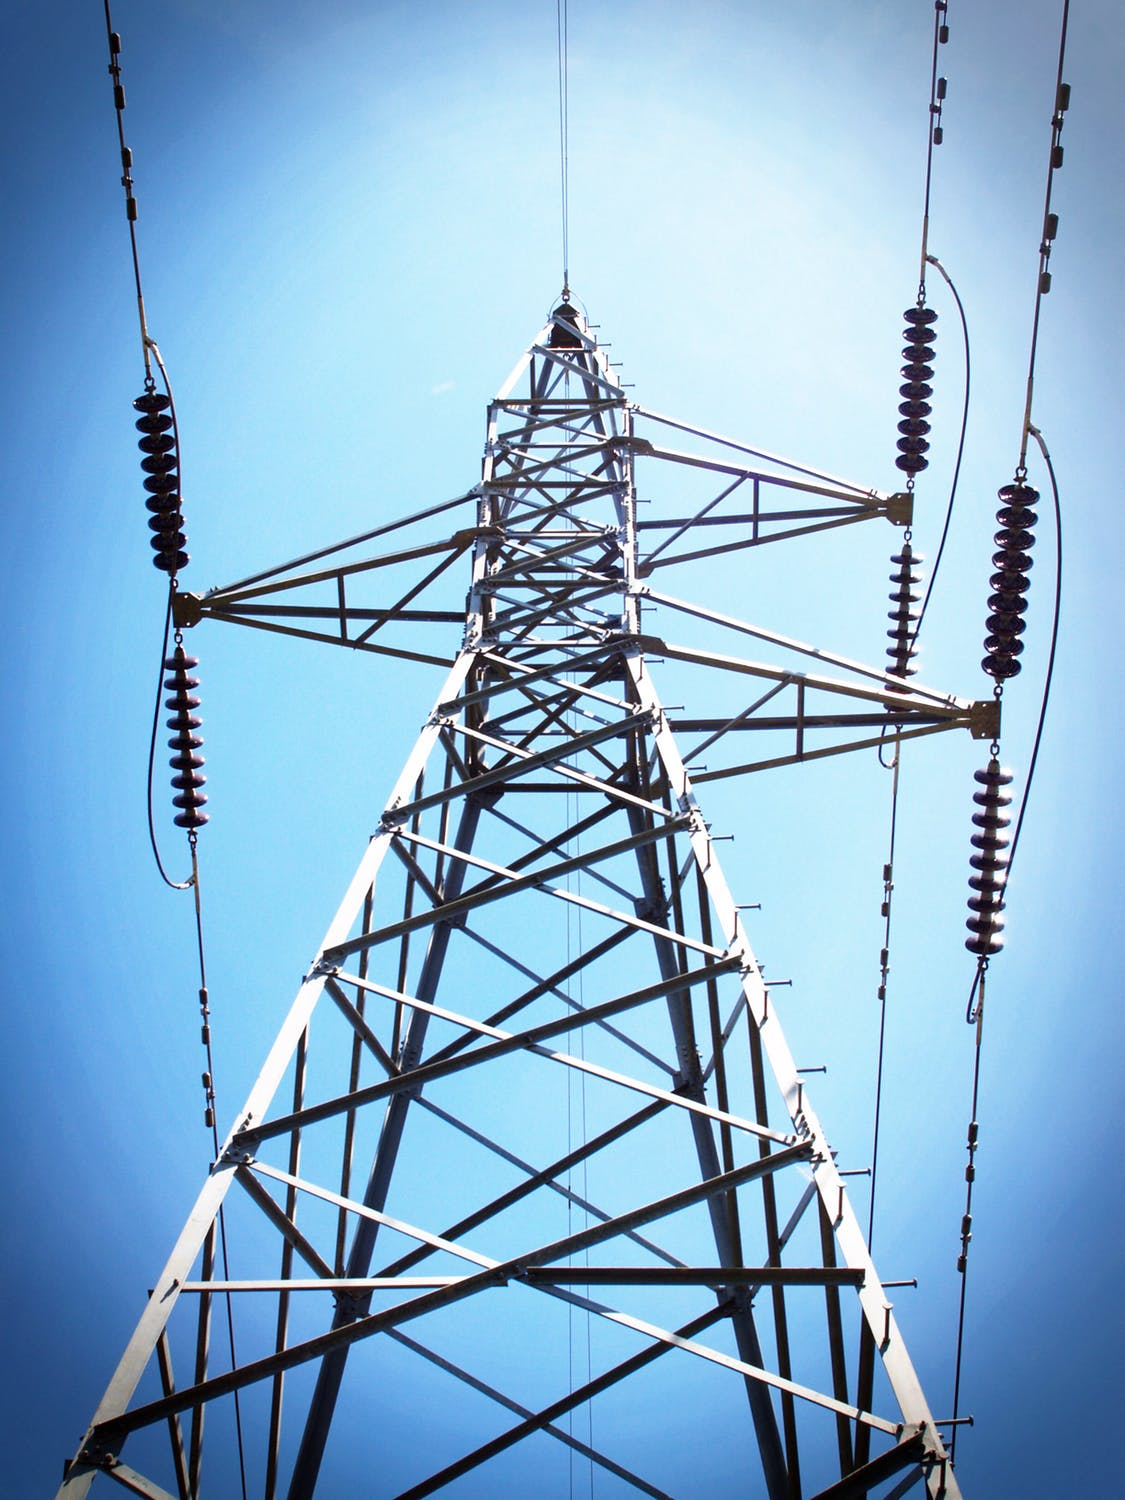
\includegraphics[scale=0.25]{rysunki/example}
\caption{Przyk�adowy obraz zamieszczony w pracy dyplomowej}
\label{img/template1}
\end{figure}
Vestibulum lorem elit, ornare vitae ultrices non, rhoncus eu elit. Vestibulum et gravida erat. Sed ut velit sollicitudin, blandit libero nec, maximus felis. Morbi feugiat pharetra lacus sit amet sodales. Aenean a sem elit. Ut et augue justo. Sed id consequat magna, non tincidunt eros. Sed congue tellus vitae ipsum commodo, nec pretium quam congue. Fusce non imperdiet sem, at imperdiet nibh. Morbi convallis nisl ante. Maecenas hendrerit, augue ac pretium molestie, ex massa lacinia est, sit amet volutpat eros magna vel erat.

Nunc egestas mauris sit amet sem facilisis, in rutrum quam faucibus. Etiam ornare fringilla tellus, sit amet bibendum nulla fermentum vitae. Nullam nec consectetur ipsum. Duis pulvinar libero vel diam lacinia, ac dapibus massa malesuada. Nullam sit amet gravida risus, nec tincidunt enim. Integer vehicula, nisl vitae hendrerit molestie, arcu arcu eleifend enim, at tempus odio leo nec nibh. Sed ut tortor risus. Nulla mattis pretium gravida. Phasellus eu augue magna. Proin quis dolor consectetur, accumsan velit et, maximus ipsum. 

Vestibulum lorem elit, ornare vitae ultrices non, rhoncus eu elit. Vestibulum et gravida erat. Sed ut velit sollicitudin, blandit libero nec, maximus felis. Morbi feugiat pharetra lacus sit amet sodales. Aenean a sem elit. Ut et augue justo. Sed id consequat magna, non tincidunt eros. Sed congue tellus vitae ipsum commodo, nec pretium quam congue. Fusce non imperdiet sem, at imperdiet nibh. Morbi convallis nisl ante. Maecenas hendrerit, augue ac pretium molestie, ex massa lacinia est, sit amet volutpat eros magna vel erat.

\begin{table}[ht]
\captionsetup{justification=centering}
\caption{Dane techniczne silnika nap�dowego uk�adu jezdnego}
\centering
    \begin{tabular}{|l|l|c|}
    \hline
    \multicolumn{1}{|l|}{\textbf{Lp.}} & \multicolumn{1}{l|}{\textbf{Parametr}} & \multicolumn{1}{c|}{\textbf{Warto��}} \\
    \hline
       1.   & Napi�cie zasilania [V] & 12  \\
    \hline
       2.   &  Pr�dko�� obrotowa [obr/min]& 200\\
    \hline
       3.  & Moment obrotowy [Nm]   & 0.8 \\
    \hline
       4.  & Maks. pr�d pracy [A]      &  0.8 \\
    \hline
       5.  & �rednica wa�u [mm]     &  8 \\
    \hline
       6.  & Rodzaj czujnika     &  Inkrementalny   \\
    \hline
       7.  & Rozdzielczo�� enkodera [imp/obr]   &  75 \\
    \hline
    \end{tabular}
  \label{silnik_skret}
\end{table}

Nunc egestas mauris sit amet sem facilisis, in rutrum quam faucibus. Etiam ornare fringilla tellus, sit amet bibendum nulla fermentum vitae. Nullam nec consectetur ipsum. Duis pulvinar libero vel diam lacinia, ac dapibus massa malesuada. Nullam sit amet gravida risus, nec tincidunt enim. Integer vehicula, nisl vitae hendrerit molestie, arcu arcu eleifend enim, at tempus odio leo nec nibh. Sed ut tortor risus. Nulla mattis pretium gravida. Phasellus eu augue magna. Proin quis dolor consectetur, accumsan velit et, maximus ipsum. 



Nunc egestas mauris sit amet sem facilisis, in rutrum quam faucibus. Etiam ornare fringilla tellus, sit amet bibendum nulla fermentum vitae. Nullam nec consectetur ipsum. Duis pulvinar libero vel diam lacinia, ac dapibus massa malesuada. Nullam sit amet gravida risus, nec tincidunt enim. Integer vehicula, nisl vitae hendrerit molestie, arcu arcu eleifend enim, at tempus odio leo nec nibh. Sed ut tortor risus. Nulla mattis pretium gravida. Phasellus eu augue magna. Proin quis dolor consectetur, accumsan velit et, maximus ipsum. 


Nunc egestas mauris sit amet sem facilisis, in rutrum quam faucibus. Etiam ornare fringilla tellus, sit amet bibendum nulla fermentum vitae. Nullam nec consectetur ipsum. Duis pulvinar libero vel diam lacinia, ac dapibus massa malesuada. Nullam sit amet gravida risus, nec tincidunt enim. Integer vehicula, nisl vitae hendrerit molestie, arcu arcu eleifend enim, at tempus odio leo nec nibh. Sed ut tortor risus. Nulla mattis pretium gravida. Phasellus eu augue magna. Proin quis dolor consectetur, accumsan velit et, maximus ipsum. 

\begin{equation}
\label{rownanie}
\sum_{n=1}^{\infty} 2^{-n} \arccos(\frac{\int_{a}^{b} x^2 dx}{x})  = 1
\end{equation}

Nunc egestas mauris sit amet sem facilisis, in rutrum quam faucibus. Etiam ornare fringilla tellus, sit amet bibendum nulla fermentum vitae. Nullam nec consectetur ipsum. Duis pulvinar libero vel diam lacinia, ac dapibus massa malesuada. Nullam sit amet gravida risus, nec tincidunt enim. Integer vehicula, nisl vitae hendrerit molestie, arcu arcu eleifend enim, at tempus odio leo nec nibh. Sed ut tortor risus. Nulla mattis pretium gravida. Phasellus eu augue magna. Proin quis dolor consectetur, accumsan velit et, maximus ipsum. 

\lstset{style=matlab}

\begin{lstlisting}[caption={Przyk�adowy listing programu Matlab}]
for n = 1 : 4
    
    for j = 1 : 100
        Imp_1_100(n,j) = (R1*R2*C2*i*j*2*pi + R1 + R2);
    end
    
    % Zmiana warto�ci  
    
    if log(abs(Imp_1_100(n,100))) - log(Rr) <= 2
        Rr = Rr/10;
    end
    
    RT(n) = Rr;  % Przypisanie warto�ci
end
\end{lstlisting}


\lstset{style=java}

\begin{lstlisting}[caption={Przyk�adowy listing w j�zyku Java},label=javovy]
class OuterClass {
  int x = 10;

  private class InnerClass {
    int y = 5;
  }
}

public class MyMainClass {
  public static void main(String[] args) {
    OuterClass myOuter = new OuterClass();
    OuterClass.InnerClass myInner = myOuter.new InnerClass();
    System.out.println(myInner.y + myOuter.x);
  }
}
\end{lstlisting}

\newpage





\lstset{style=vhdl}

\begin{lstlisting}[caption={Przyk�adowy listing w j�zyku VHDL}]

architecture FSMD of gcd is
begin

    process(rst, clk)

    -- define states using variable 
    type S_Type is (ST0, ST1, ST2);
    variable State: S_Type := ST0 ;			
    variable Data_X, Data_Y: unsigned(3 downto 0);
	
    begin

        if (rst='1') then		    -- initialization
	    d_o <= "0000";
	    State := ST0;
	elsif (clk'event and clk='1') then
	    case State is
	        when ST0 =>		    -- starting
		    if (go_i='1') then
			Data_X := x_i;
			Data_Y := y_i;
			State := ST1;
		    else
		        State := ST0;
		    end if;
		when ST1 =>		    -- idle state 
		    State := ST2;
		when ST2 =>		    -- computation
		    if (Data_X/=Data_Y) then
		        if (Data_X<Data_Y) then
			    Data_Y := Data_Y - Data_X;
			else
			    Data_X := Data_X - Data_Y;
			end if;
			State := ST1;
		    else
			d_o <=Data_X;       -- done
		        State := ST0;
		    end if;
		when others =>		    -- go back 
		    d_o <= "ZZZZ";
		    State := ST0;
            end case;				
 	end if;
    
    end process;		

end FSMD;

\end{lstlisting}


Nunc egestas mauris sit amet sem facilisis, in rutrum quam faucibus. Etiam ornare fringilla tellus, sit amet bibendum nulla fermentum vitae. Nullam nec consectetur ipsum. Duis pulvinar libero vel diam lacinia, ac dapibus massa malesuada. Nullam sit amet gravida risus, nec tincidunt enim. Integer vehicula, nisl vitae hendrerit molestie, arcu arcu eleifend enim, at tempus odio leo nec nibh. Sed ut tortor risus. Nulla mattis pretium gravida. Phasellus eu augue magna. Proin quis dolor consectetur, accumsan velit et, maximus ipsum. 
Nunc egestas mauris sit amet sem facilisis, in rutrum quam faucibus. Etiam ornare fringilla tellus, sit amet bibendum nulla fermentum vitae. Nullam nec consectetur ipsum. Duis pulvinar libero vel diam lacinia, ac dapibus massa malesuada. Nullam sit amet gravida risus, nec tincidunt enim. Integer vehicula, nisl vitae hendrerit molestie, arcu arcu eleifend enim, at tempus odio leo nec nibh. Sed ut tortor risus. Nulla mattis pretium gravida. Phasellus eu augue magna. Proin quis dolor consectetur, accumsan velit et, maximus ipsum. 

Nunc egestas mauris sit amet sem facilisis, in rutrum quam faucibus. Etiam ornare fringilla tellus, sit amet bibendum nulla fermentum vitae. Nullam nec consectetur ipsum. Duis pulvinar libero vel diam lacinia, ac dapibus massa malesuada. Nullam sit amet gravida risus, nec tincidunt enim. Integer vehicula, nisl vitae hendrerit molestie, arcu arcu eleifend enim, at tempus odio leo nec nibh. Sed ut tortor risus. Nulla mattis pretium gravida. Phasellus eu augue magna. Proin quis dolor consectetur, accumsan velit et, maximus ipsum. 



% Definition of blocks:
\tikzset{%
  block/.style    = {draw, thick, rectangle, minimum height = 3em,
    minimum width = 3em},
  sum/.style      = {draw, circle, node distance = 2cm}, % Adder
  input/.style    = {coordinate}, % Input
  output/.style   = {coordinate} % Output
}
% Defining string as labels of certain blocks.
\newcommand{\suma}{\Large$+$}
\newcommand{\inte}{$\displaystyle \int$}
\newcommand{\derv}{\huge$\frac{d}{dt}$}

\begin{figure}[ht]

\begin{tikzpicture}[auto, thick, node distance=2cm, >=triangle 45]
\draw
	% Drawing the blocks of first filter :
	node at (0,0)[right=-3mm]{\Large }
	node [input, name=input1] {} 
	node [sum, right of=input1] (suma1) {\suma}
	node [block, right of=suma1] (inte1) {\inte}
         node at (6.8,0)[block] (Q1) {\Large $Q_1$}
         node [block, below of=inte1] (ret1) {\Large$T_1$$$};
    % Joining blocks. 
    % Commands \draw with options like [->] must be written individually
	\draw[->](input1) -- node {$X(Z)$}(suma1);
 	\draw[->](suma1) -- node {} (inte1);
	\draw[->](inte1) -- node {} (Q1);
	\draw[->](ret1) -| node[near end]{} (suma1);
	% Adder
\draw
	node at (5.4,-4) [sum, name=suma2] {\suma}
    	% Second stage of filter 
	node at  (1,-6) [sum, name=suma3] {\suma}
	node [block, right of=suma3] (inte2) {\inte}
	node [sum, right of=inte2] (suma4) {\suma}
	node [block, right of=suma4] (inte3) {\inte}
	node [block, right of=inte3] (Q2) {\Large$Q_2$$$}
	node at (9,-8) [block, name=ret2] {\Large$T_2$$$}
;
	% Joining the blocks of second filter
	\draw[->] (suma3) -- node {} (inte2);
	\draw[->] (inte2) -- node {} (suma4);
	\draw[->] (suma4) -- node {} (inte3);
	\draw[->] (inte3) -- node {} (Q2);
	\draw[->] (ret2) -| (suma3);
	\draw[->] (ret2) -| (suma4);
         % Third stage of filter:
	% Defining nodes:
\draw
	node at (11.5, 0) [sum, name=suma5]{\suma}
	node [output, right of=suma5]{}
	node [block, below of=suma5] (deriv1){\derv}
	node [output, right of=suma5] (sal2){}
;
	% Joining the blocks:
	\draw[->] (suma2) -| node {}(suma3);
	\draw[->] (Q1) -- (8,0) |- node {}(ret1);
	\draw[->] (8,0) |- (suma2);
	\draw[->] (5.4,0) -- (suma2);
	\draw[->] (Q1) -- node {}(suma5);
	\draw[->] (deriv1) -- node {}(suma5);
	\draw[->] (Q2) -| node {}(deriv1);
    	\draw[<->] (ret2) -| node {}(deriv1);
    	\draw[->] (suma5) -- node {$Y(Z)$}(sal2);
    	% Drawing nodes with \textbullet
\draw
	node at (8,0) {\textbullet} 
	node at (8,-2){\textbullet}
	node at (5.4,0){\textbullet}
    	node at (5,-8){\textbullet}
    	node at (11.5,-6){\textbullet}
    	;
	% Boxing and labelling noise shapers
	\draw [color=gray,thick](-0.5,-3) rectangle (9,1);
	\node at (-0.5,1) [above=5mm, right=0mm] {\textsc{generator szumu I rz�du}};
	\draw [color=gray,thick](-0.5,-9) rectangle (12.5,-5);
	\node at (-0.5,-9) [below=5mm, right=0mm] {\textsc{generator szumu II rz�du}};
\end{tikzpicture}
\caption{Przyk�adowy schemat blokowy utworzony przy u�yciu pakietu tikz}
\end{figure}

Nunc egestas mauris sit amet sem facilisis, in rutrum quam faucibus. Etiam ornare fringilla tellus, sit amet bibendum nulla fermentum vitae. Nullam nec consectetur ipsum. Duis pulvinar libero vel diam lacinia, ac dapibus massa nc egestas mauris sit amet sem facilisis, in rutrum quam faucibus. Etiam ornare fringilla tellus, sit amet bibendum nulla fermentum vitae. Nullam nec consectetur ipsum. Duis pulvinar libero vel diam lacinia, ac dapibus massa.




\chapter{Analiza techniczna}
\autsection{Wprowadzenie}{Agnieszka Wojciechowska}
Analiza techniczna to narz�dzie s�u��ce do analizy wykres�w gie�dowych, kt�ra ma na celu prognoz� przysz�ych cen kurs�w na podstawie historycznych zmian cen. Modele analizy technicznej charakteryzuj� pewne powtarzalne schematy mo�liwe do zaobserwowania w zmianach cen akcji. W zale�no�ci od danego modelu mo�na zaobserwowa� powtarzalne zachowanie wska�nik�w statystycznych. [11]

Na wst�pie zostanie om�wiony jeden z popularniejszych narz�dzi na polskim rynku pozwalaj�cy na analiz� techniczn� wybranych wykres�w. W kolejnych rozdzia�ach zosta�y zaprezentowane zasady dzia�ania wska�nik�w stosowanych w analizie technicznej i ich przyk�ady, kt�re zosta�y zaimplementowane w projekcie. Do zdefiniowania narz�dzi analizy technicznej zostanie u�yta wiedza przedstawiona w poprzednim rozdziale.

\subsection{Analiza rynkowa}
Istnieje bardzo du�o narz�dzi w obszarze analizy technicznej wykorzystywanych na rynku finansowym. Na polskim rynku jednym z bardziej popularnych jest aplikacja ''BiznesRadar'' dost�pna w mobilnej wersji oraz online. Ma ona pomaga� inwestorom w podejmowaniu decyzji o transakcji, wspiera� ich strategi� inwestycyjn� lub s�u�y� do analizowania notowa� na rynku na podstawie przesz�ych danych. 
\begin{figure*}[!h]
  % wy�rodkowanie zawarto�ci pola obrazka
  \begin{center}
    % okienko skaluj�ce:
    %  pierwszy argument szeroko��, drugi wysoko��,
    %  jeden z nich mo�e by� zast�piony ! - zachowanie proporcji obrazka
    %  w taki spos�b mo�emy skalowa� tak�e inne obiekty np. tekst
    \resizebox{1\textwidth}{!}{
      % wstawienie obrazka
      \includegraphics{rysunki/Biznes_Radar}
    }
    % opis obrazka
    \caption[aplikacja BiznesRadar - logo {[12]}]{Logo aplikacji BiznesRadar dost�pnej w sklepie Google.}
    % etykieta
    \label{BiznesRadar}
  \end{center}
\end{figure*}

Aplikacja ''Biznes Radar'' stworzona przez sp�k� o tej samej nazwie umo�liwia u�ytkownikowi �ledzenie wskaza� w�asnych inwestycji i notowania kurs�w. S� one synchronizowane z rzeczywistym Domem Maklerskim poprzez portal BiznesRadar.pl [2]. 

Jest to narz�dzie skierowane do inwestor�w, g��wnie do�wiadczonych. Do�wiadczonych oznacza takich inwestor�w, kt�rzy potrafi� czyta� przedstawione wykresy oraz maj� podstawow� wiedz� na temat dost�pnych narz�dzi i instrument�w na rynku.

\begin{figure*}[!h]
  % wy�rodkowanie zawarto�ci pola obrazka
  \begin{center}
    % okienko skaluj�ce:
    %  pierwszy argument szeroko��, drugi wysoko��,
    %  jeden z nich mo�e by� zast�piony ! - zachowanie proporcji obrazka
    %  w taki spos�b mo�emy skalowa� tak�e inne obiekty np. tekst
    \resizebox{0.8\textwidth}{!}{
      % wstawienie obrazka
      \includegraphics{rysunki/Biznes_Radar_wskazniki}
      \includegraphics{rysunki/Biznes_Radar_wykres}
    }
    % opis obrazka
    \caption[aplikacja BiznesRadar - indeksy i wykres {[12]}]{Rysunek przedstawia dwa ekrany wewn�trz aplikacji BiznesRadar. Po prawej przedstawione s� dost�pne indeksy do analizy notowa�. Po lewej przedstawiony jest wygenerowany wykres cen dla sp�ki KGH Polska Mied�. [12]}
    % etykieta
    \label{BiznesRadar}
  \end{center}
\end{figure*}

Ponad to, jak pokazano na rys. 4.3  narz�dzie zawiera ekran, w kt�rym przedstawione s� podsumowane warto�ci wska�nik�w i ich interpretacje za pomoc� oceny kupuj/ neutralnie / sprzedaj. Odpowiedni zysk inwestora jest te� przedstawiany w kompleksowym sprawozdaniu z portfela.
\begin{figure*}[!h]
  % wy�rodkowanie zawarto�ci pola obrazka
  \begin{center}
    % okienko skaluj�ce:
    %  pierwszy argument szeroko��, drugi wysoko��,
    %  jeden z nich mo�e by� zast�piony ! - zachowanie proporcji obrazka
    %  w taki spos�b mo�emy skalowa� tak�e inne obiekty np. tekst
    \resizebox{0.8\textwidth}{!}{
      % wstawienie obrazka
      \includegraphics{rysunki/Biznes_Radar_odp}
      \includegraphics{rysunki/Biznes_Radar_zysk}
    }
    % opis obrazka
    \caption[aplikacja BiznesRadar - decyzje i sprawozdania {[12]}]{Rysunek przedstawia dwa ekrany wewn�trz aplikacji BiznesRadar. Po prawej znajduje si� lista wzka�nik�w oraz ich warto�� i ocena. Po lewej znajduje si� ekran ze sprawozdaniem z portfela inwestycyjnego danego u�ytkownika z podsumowaniem zysk�w.[12]}
    % etykieta
    \label{BiznesRadar}
  \end{center}
\end{figure*}


\autsection{MACD}{Agnieszka Wojciechowska}
\subsection{wprowadzenie}
MACD to skr�t od Moving Average Convergence Divergence co w polskim t�umaczeniu oznacza zbie�no�� i rozbie�no�� �redniej krocz�cej.

Wska�nik ten zosta� opracowany przez Geralda Appel'a w roku 1970. Opracowa� on fundamentaln� w�aciwo�� tego wska�nika, czyli interpretacj� i przewidywanie przeci�� linii MACD. Nast�pnie w roku 1986 dodany zosta� histogram przez Thomasa Aspray'a, kt�re umo�liwi�o obserwacj� impetu ceny. [15]

Aktualnie MACD jest jednym z najpoplarniejszych wska�nik�w stosowanych w analizie technicznej. Zawdzi�cza to dzi�ki temu, �e jest �atwy w interpretacji sygna��w oraz dzi�ki mo�liwo�ci zastosowania go w r�nych warunkach rynkowych - zar�wno stablilnej, jak i w trakcie nag�ych wzrost�w, b�d� spadk�w cen.
\subsection{zasady dzia�ania}
\subsubsection{wz�r}
Tym co wyr�nia wska�nik MACD jest po��czenie dw�ch r�nych typ�w wska�nik�w. Wz�r wska�nika wyznacza sygna�y kupna, b�d� sprzeda�y na podstawie dw�ch linii zwanych lini� macd i lini� sygna�ow�.

Do wyznaczenia linii MACD wykorzystywana jest r�nica dw�ch �rednich ruchomych sygna�u wejciowego X, o r�nych okresach. Standardowo przyjmowane s� 26 i 12 okresowe przedzia�y �redniej wyk�adniczej, jest to ustawienie domylne. Linia MACD s�u�y do identyfikacji kierunku i czasu trwania trendu. 

Nast�pnie linia signal wyliczana jest na podstawie najcz�ciej 9 okresowej �redniej wyk�adniczej z linii MACD.  [13] [15] [16]
\begin{equation}
\begin{array}{rcl}
MACD & = & EMA_{26}(X) - EMA_{12}(X) \\
signal & = & EMA_{9}(MACD)
\end{array}
\end{equation}
We wzorze:
\begin{itemize}
\item $EMA_{X}$ - �rednia krocz�ca wyk�adniczo w przedziale X okresowym, X - dowolna liczba naturalna
\end{itemize}
\subsubsection{strategia decyzyjna}
Strategia MACD opiera si� g��wnie o interpretacj� przeci�� linii sygna�u z lini� MACD. Analiza przeci�� wygl�da w nast�puj�cy spos�b:
\begin{itemize}
    \item Sygna� na kupno akcji - linia MACD przecina lini� signal od do�u
    \item Sygna� na sprzeda� akcji - linia MACD przecina lini� signal od g�ry
\end{itemize}
Na poni�szym wykresie (rys. 4.4) zosta�y zaznaczone omawiane linie wska�nika MACD. Mo�na zauwa�y� wyra�ne momenty przecinania si� sygna��w.
\begin{figure*}[!h]
  % wy�rodkowanie zawarto�ci pola obrazka
  \begin{center}
    % okienko skaluj�ce:
    %  pierwszy argument szeroko��, drugi wysoko��,
    %  jeden z nich mo�e by� zast�piony ! - zachowanie proporcji obrazka
    %  w taki spos�b mo�emy skalowa� tak�e inne obiekty np. tekst
    \resizebox{1\textwidth}{!}{
      % wstawienie obrazka
      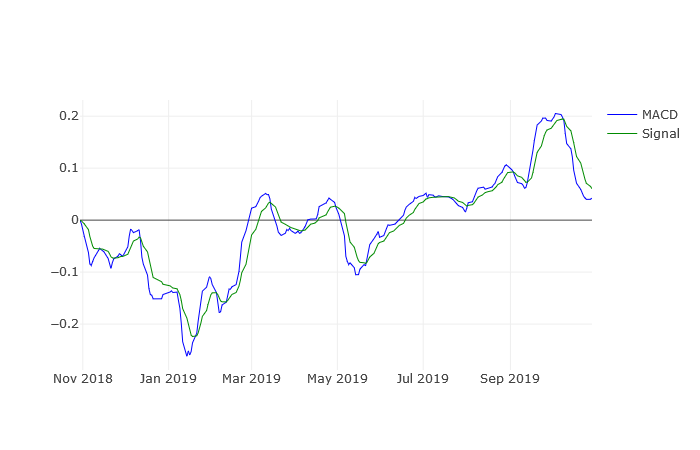
\includegraphics{rysunki/MACD}
    }
    % opis obrazka
    \caption[wykres MACD]{Wykres przedstawia linie MACD oraz signal.}
    % etykieta
    \label{Wykres MACD}
  \end{center}
\end{figure*}

Od odpowiedniej interpretacji sygna��w zale�y r�wnie� fakt przeci�cia linii zero oraz odleg�o�� od tej linii. W momencie gdy sygna� kupna jest generowany znacz�co poni�ej linii zero to jest on interpretowany jako bardziej wiarygodny. Czym wi�ksza jest w�a�nie odleg�o�� od linii zera, tym wi�ksza wiarygodno��. R�wnie� tym wi�ksze jest prawdopodobie�stwo kontynuowania ruchu spadkowego. Analogicznie dzieje si� dla sygna�u sprzeda�y gdy sygna� ten jest generowany znacz�co powy�ej linii zero. [13] [15]

Interpretacj� wska�nika MACD mo�na wzbogaci� o analiz� histogramu MACD. Dzi�ki tej funkcjonalno�ci mo�na zaobserwowa� lokalne szczyty cenowe dla warto�ci histogramu powy�ej zera. Analogicznie dla warto�ci kszta�tuj�cych si� poni�ej zera obserwuje si� do�ki cenowe. Szersza interpretacja histogramu nie b�dzie omawiana, gdy� opisywana aplikacja nie uwzgl�dnia tej funkcjonalno�ci. [13]

Oczywi�cie tak jak w przypadku ka�dego innego wska�nika sygna� kupna czy sprzeda�y nie daje �adnej gwarancji, �e zyskamy na transakcji.

\subsection{przyk�ady numeryczne}
\begin{figure*}[!h]
  % wy�rodkowanie zawarto�ci pola obrazka
  \begin{center}
    % okienko skaluj�ce:
    %  pierwszy argument szeroko��, drugi wysoko��,
    %  jeden z nich mo�e by� zast�piony ! - zachowanie proporcji obrazka
    %  w taki spos�b mo�emy skalowa� tak�e inne obiekty np. tekst
    \resizebox{1\textwidth}{!}{
      % wstawienie obrazka
      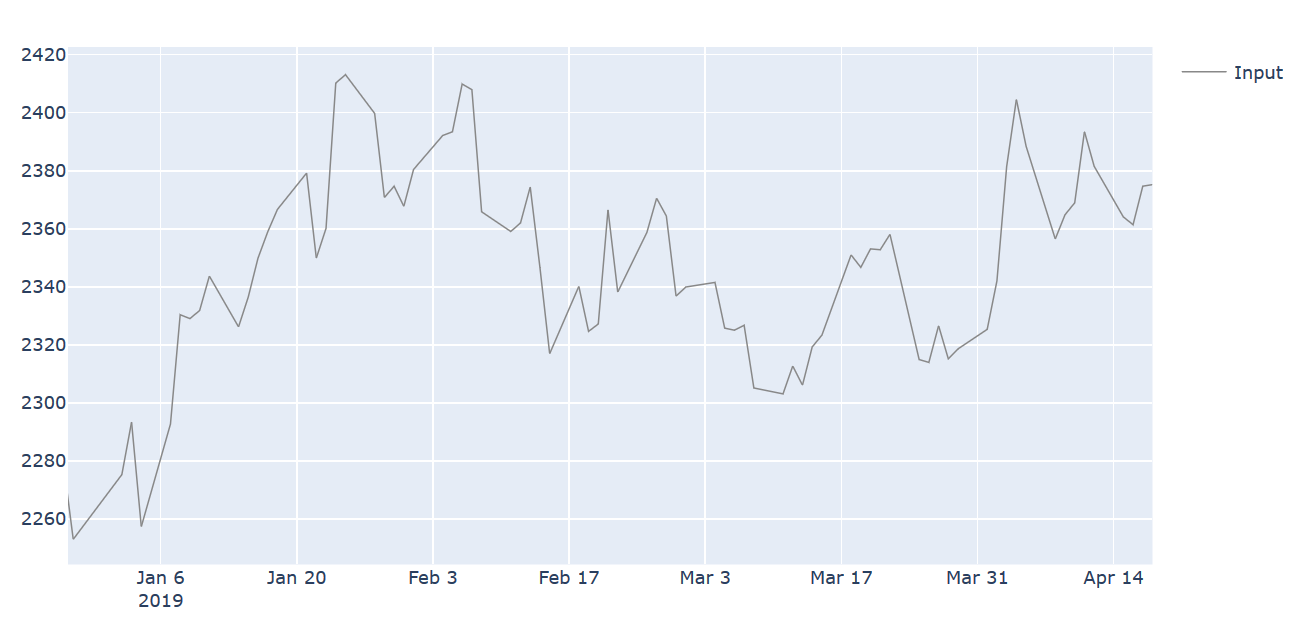
\includegraphics{rysunki/input_MACD_stochastic}
    }
    % opis obrazka
    \caption[MACD - sygnal wejsciowy]{Wykres przedstawia sygna� wej�ciowy do przedstawionych poni�ej przyk�ad�w MACD.}
    % etykieta
    \label{MACD - sygnal wejsciowy}
  \end{center}
\end{figure*}

Zastosowanie i interpretacja wska�nika MACD w praktyce zostanie przedstawiona na dw�ch poni�szych przyk�adach. Do przyk�adu, dla wi�kszej czytelno�ci wykresu zosta�o wybrane przybli�enie warto�ci do zakresu 4 miesi�cy, od stycznia do kwietnia 2019. Ponadto u�yte dane pochodz� z serwisu Stooq [17]. Dane wej�ciowe zosta�y przedstawione na rys. 4.5.

\subsubsection{Przyk�ad 1: sygna� kupna}
Dla sygna�u kupna oznaczonego na rys. 4.2 liter� "K" linia MACD (niebieska) przecina lini� signal (zielona) od do�u. W tym przyk�adzie mo�na zaobserwowa� cztery wygenerowane przyk�ady sygna��w kupna: 8 stycznia, 7 lutego, 18 marca i 2 kwietnia.
\begin{figure*}[!h]
  % wy�rodkowanie zawarto�ci pola obrazka
  \begin{center}
    % okienko skaluj�ce:
    %  pierwszy argument szeroko��, drugi wysoko��,
    %  jeden z nich mo�e by� zast�piony ! - zachowanie proporcji obrazka
    %  w taki spos�b mo�emy skalowa� tak�e inne obiekty np. tekst
    \resizebox{1\textwidth}{!}{
      % wstawienie obrazka
      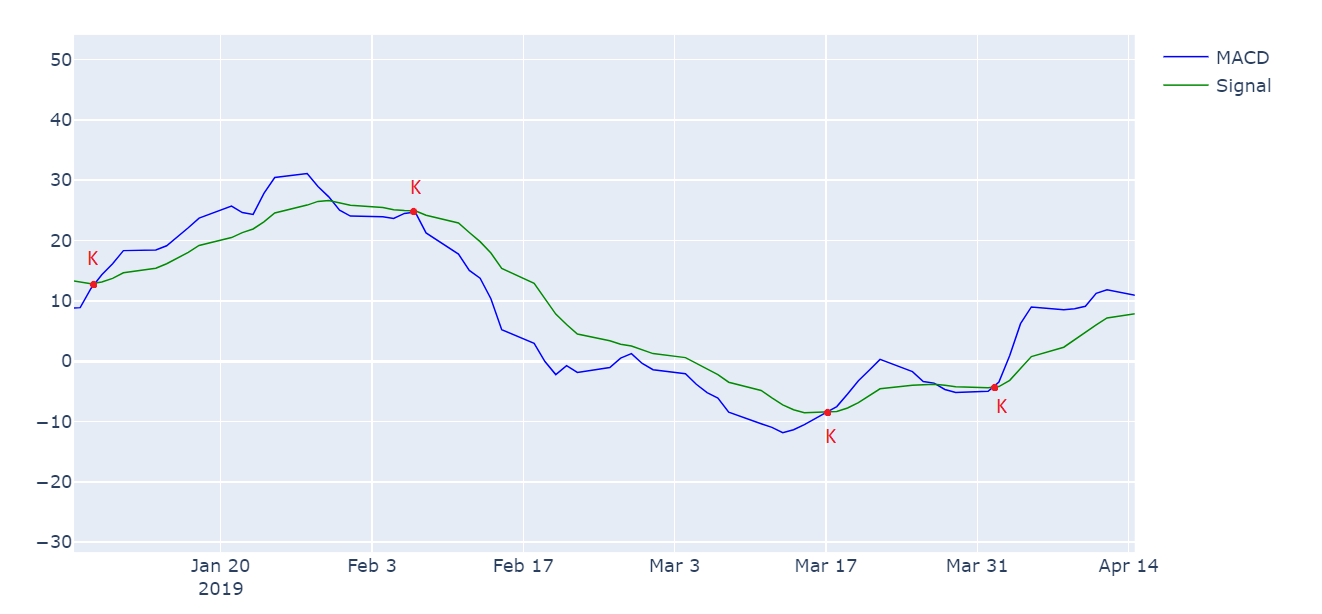
\includegraphics{rysunki/MACD_kup}
    }
    % opis obrazka
    \caption[MACD - sygna�y kupna]{Wykres przedstawia sygna�y kupna (K) wygenerowane przez wska�nik MACD.}
    % etykieta
    \label{Wykres MACD}
  \end{center}
\end{figure*}

Jednym z d�u�szych okres�w, gdy linia MACD znajdowa�a si� nad lini� signal jest pierwszy przypadek, to jest od 8 stycznia. Niestety jest to niewiarygodny sygna�, poniewa� znajduje si� powy�ej linii 0. Tak samo jest dla wskazania z 7 lutego.

Dla por�wnania sygna�y kupna po prawej stronie wykresu, to jest z dnia 18 marca i 2 kwietnia zosta�y wygenerowane poni�ej linii 0. Oznacza to, �e sygna� ten jest wiarygodny. Najbardziej wiarygodny sygna� kupna w tym przypadku zosta� wygenerowany w�a�nie 18 marca. W kolejnych dniach ta wiarygodno�� maleje, bo do 20 marca wzrasta w kierunku linii 0. Podobnie dzieje si� po 2 kwietnia. W momencie gdy sygna� przekroczy lini� 0 sygna� kupna staje si� niewiarygodny. [14]

\subsubsection{Przyk�ad 2: sygna� sprzeda�y}
Z kolei dla sygna�u sprzeda�y oznaczonego na rys. 4.3 liter� "S" linia MACD (niebieska) przecina lini� signal (zielona) od g�ry. W tym przyk�adzie mo�na zaobserwowa� dwa wygenerowane przyk�ady sygna��w sprzeda�y: 30 stycznia i 27 marca.
\begin{figure*}[!h]
  % wy�rodkowanie zawarto�ci pola obrazka
  \begin{center}
    % okienko skaluj�ce:
    %  pierwszy argument szeroko��, drugi wysoko��,
    %  jeden z nich mo�e by� zast�piony ! - zachowanie proporcji obrazka
    %  w taki spos�b mo�emy skalowa� tak�e inne obiekty np. tekst
    \resizebox{1\textwidth}{!}{
      % wstawienie obrazka
      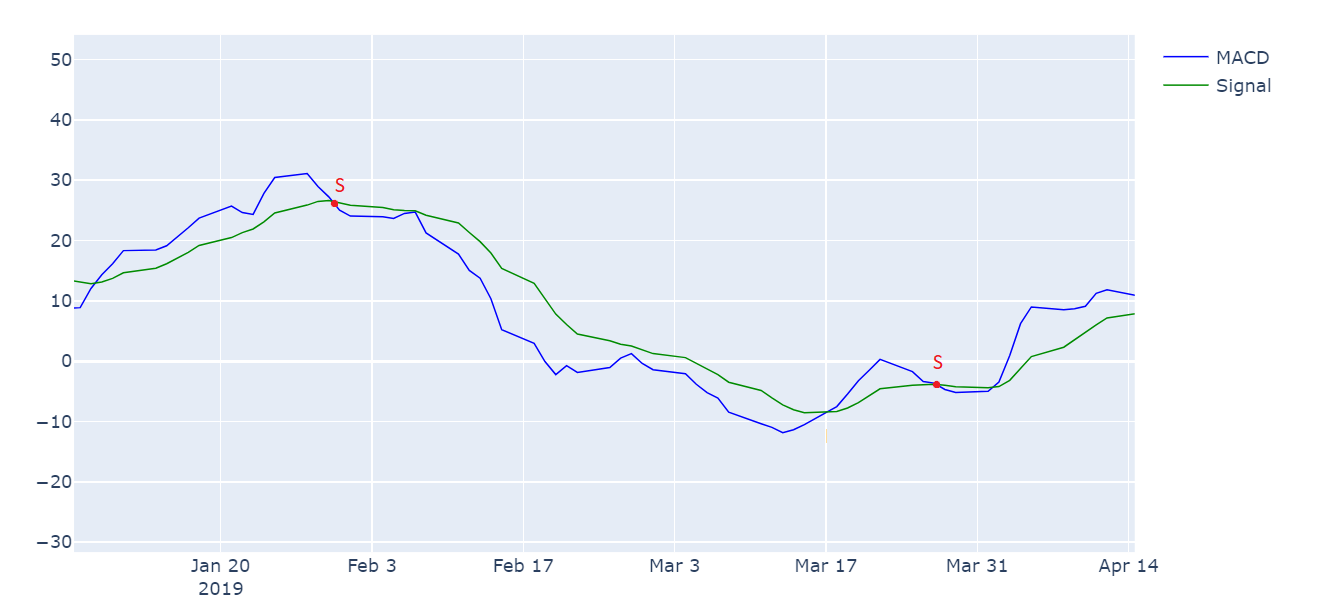
\includegraphics{rysunki/MACD_sprzedaj}
    }
    % opis obrazka
    \caption[MACD - sygna�y sprzeda�y]{Wykres przedstawia sygna�y sprzeda�y (S) wygenerowane przez wska�nik MACD.}
    % etykieta
    \label{Wykres MACD}
  \end{center}
\end{figure*}

Pocz�tkowo sygna� sprzeda�y wygenerowany dnia 30 stycznia jest wiarygodny, poniewa� znajduje si� wysoko ponad lini� 0. Z biegiem czasu wskazania spadaj� w kierunku linii 0. Gdy przekracza on t� lini� 19 lutego sygna� staje si� niewiarygodny. Najwi�ksz� wiarygodno�� w ca�ym analizowanym zakresie 4 miesi�cy wska�nik osi�ga 30 stycznia.

Drugi wygenerowany sygna� z dnia 27 marca jest sygna�em niewiarygodnym, gdy� znajduje si� znacz�co poni�ej linii 0. [14]
\subsection{podsumowanie}
MACD s�u�y do wszechstronnej analizy, poniewa� za jego pomoc� mo�na interpretowa� nie tylko sygna�y spadkowe i rosn�ce, ale tak�e umo�liwia �ledzenie potencjalnych do�k�w lub szczyt�w cenowych.

Generalnie wska�nik MACD znajduje najlepsze zastosowanie w �rednim oraz d�ugim terminie, poniewa� powsta� w celu wykorzystania go do odczytywania sygna��w w raz w ci�gu dnia, czyli na tak zwanym wykresie dziennym. Przy mniejszych okresach mo�e jednak powodowa� op�nione sygna�y.

\autsection{Wst�gi Bollingera}{Mateusz Rutkiewicz}
\subsection{wprowadzenie}
\begin{figure*}[!h]
  % wy�rodkowanie zawarto�ci pola obrazka
  \begin{center}
    % okienko skaluj�ce:
    %  pierwszy argument szeroko��, drugi wysoko��,
    %  jeden z nich mo�e by� zast�piony ! - zachowanie proporcji obrazka
    %  w taki spos�b mo�emy skalowa� tak�e inne obiekty np. tekst
    \resizebox{\textwidth}{!}{
      % wstawienie obrazka
      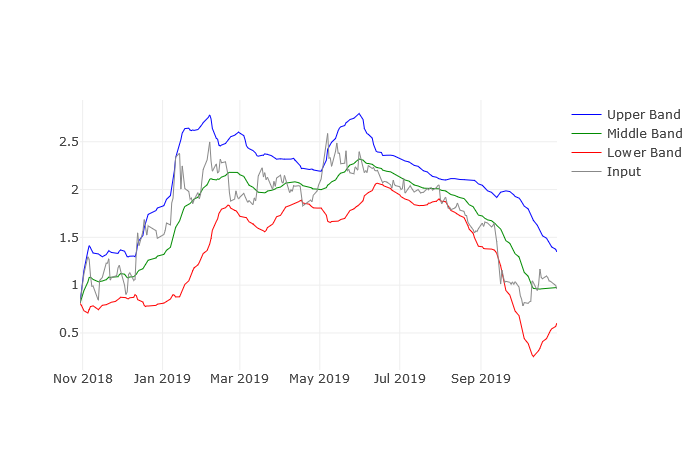
\includegraphics{rysunki/Bollinger Bands}
    }
    % opis obrazka
    \caption[Wst�gi Bollingera]{Przedstawia wykres wst�g bollingera wraz z sygna�em wej�ciowym Input.}

    % etykieta
    \label{Wykres wst�g Bollingera}
  \end{center}
\end{figure*}
Wst�gi Bollingera s� wska�nikiem opracowanym przez Johna Bollingera w latach 80. XX wieku. Sk�adaj� si� one z trzech wst�g - g�rnej wst�gi, �rodkowej wst�gi i dolnej wst�gi (ang. upper band, middle band, bottom band) i s�u�� do wykrywania do�k�w i szczyt�w cenowych. Je�eli cena znajduje si� przy dolnej wst�dze, oznacza to do�ek cenowy, a je�el znajduje si� przy g�rnej wst�dze, oznacza to szczyt cenowy.
\newpage
\subsection{zasady dzia�ania}
\subsubsection{wz�r}
�rodkowa wst�ga jest zwyk�� �redni� krocz�c� SMA z ostatnich $n$ pr�bek sygna�u $X$. G�rna wst�ga to suma �rodkowej wst�gi wraz z k-krotno�ci� odchylenia standardowego $\sigma^2$ z $n$ ostatnich pr�bek, natomiast dolna wst�ga to r�nica �rodkowej wst�gi i k-krotno�ci odchylenia standardowego z $n$ ostatnich pr�bek.
\begin{equation}
\begin{array}{rcl}
upper \: band_{(n, k)}(X) & = & SMA_{n}(X) + k\cdot\sigma_{n}(X) \\
middle \: band_{(n, k)}(X) & = & SMA_{n}(X) \\
bottom \: band_{(n, k)}(X) & = & SMA_{n}(X) - k\cdot\sigma_{n}(X),
\end{array}
\end{equation}
 Najcz�ciej stosowane parametry to $n=20$ oraz $k=2$.
\subsubsection{strategia decyzyjna}
Wst�gi Bollingera interpretuje si� w nast�puj�cy spos�b:
\begin{itemize}
    \item Sygna� na kupno akcji - sygna� wej�ciowy zbli�a si� do dolnej wst�gi b�d� jest pod ni� (wtedy jest du�a szansa, �e cena akcji zacznie rosn��)
    \item Sygna� na sprzeda� akcji - sygna� wej�ciowy zbli�a si� do g�rnej wst�gi b�d� jest nad ni� (wtedy jest du�a szansa, �e cena akcji zacznie spada�)
\end{itemize}
\newpage
\subsection{przyk�ady numeryczne}
Zastosowanie i interpretacja Wst�g Bollingera zostanie przedstawiona na trzech poni�szych przyk�adach.
\subsubsection{Przyk�ad 1: kupno w do�ku cenowym i sprzeda� w szczycie cenowym}
Przy tej strategii akcje kupuje si�, gdy cena spadnie poni�ej dolnej wst�gi, a sprzedaje si�, gdy b�dzie powy�ej g�rnej wst�gi.
\begin{figure*}[!h]
  % wy�rodkowanie zawarto�ci pola obrazka
  \begin{center}
    % okienko skaluj�ce:
    %  pierwszy argument szeroko��, drugi wysoko��,
    %  jeden z nich mo�e by� zast�piony ! - zachowanie proporcji obrazka
    %  w taki spos�b mo�emy skalowa� tak�e inne obiekty np. tekst
    \resizebox{0.75\textwidth}{!}{
      % wstawienie obrazka
      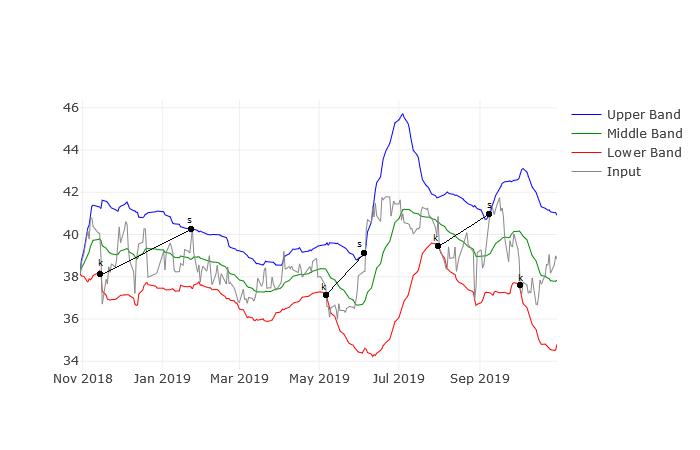
\includegraphics{rysunki/Bollinger Bands_l-u}
    }
    % opis obrazka
    \caption[Wst�gi Bollingera - Przyk�ad 1]{Wykres przedstawiaj�cy Przyk�ad 1: kupno w do�ku cenowym i sprzeda� w szczycie cenowym. Czarnym kropkami zaznaczone s� momenty kupna/sprzeda�y (literka "k" dla kupna, a  "s" dla sprzedarzy).}

    % etykieta
    \label{Wykres wst�g Bollingera}
  \end{center}
\end{figure*}
\subsubsection{Przyk�ad 2: kupno w do�ku cenowym i sprzeda� po wyj�ciu z do�ku cenowego}
Przy tej strategii akcje kupuje si�, gdy cena spadnie poni�ej dolnej wst�gi, a sprzedaje sie, gdy b�dzie powy�ej �rodkowej wst�gi.
\begin{figure*}[!h]
  % wy�rodkowanie zawarto�ci pola obrazka
  \begin{center}
    % okienko skaluj�ce:
    %  pierwszy argument szeroko��, drugi wysoko��,
    %  jeden z nich mo�e by� zast�piony ! - zachowanie proporcji obrazka
    %  w taki spos�b mo�emy skalowa� tak�e inne obiekty np. tekst
    \resizebox{0.75\textwidth}{!}{
      % wstawienie obrazka
      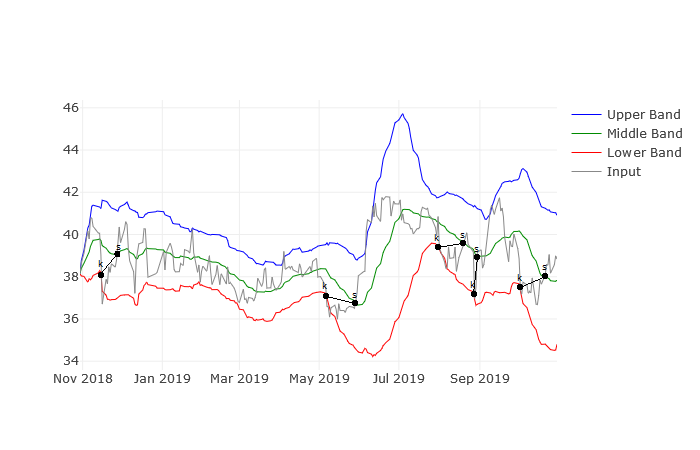
\includegraphics{rysunki/Bollinger Bands_l-m}
    }
    % opis obrazka
    \caption[Wst�gi Bollingera - Przyk�ad 2]{Wykres przedstawiaj�cy Przyk�ad 2: kupno w do�ku cenowym i sprzeda� po wyj�ciu z do�ku cenowego. Czarnym kropkami zaznaczone s� momenty kupna/sprzeda�y (literka "k" dla kupna, a  "s" dla sprzedarzy).}

    % etykieta
    \label{Wykres wst�g Bollingera}
  \end{center}
\end{figure*}
\subsubsection{Przyk�ad 3: sprzeda� w szczycie cenowym i kupno po wyj�ciu ze szczytu cenowego}
Przy tej strategii akcje kupuje si�, gdy cena spadnie poni�ej �rodkowej wst�gi, a sprzedaje sie, gdy b�dzie powy�ej g�rnej wst�gi.
\begin{figure*}[!h]
  % wy�rodkowanie zawarto�ci pola obrazka
  \begin{center}
    % okienko skaluj�ce:
    %  pierwszy argument szeroko��, drugi wysoko��,
    %  jeden z nich mo�e by� zast�piony ! - zachowanie proporcji obrazka
    %  w taki spos�b mo�emy skalowa� tak�e inne obiekty np. tekst
    \resizebox{0.75\textwidth}{!}{
      % wstawienie obrazka
      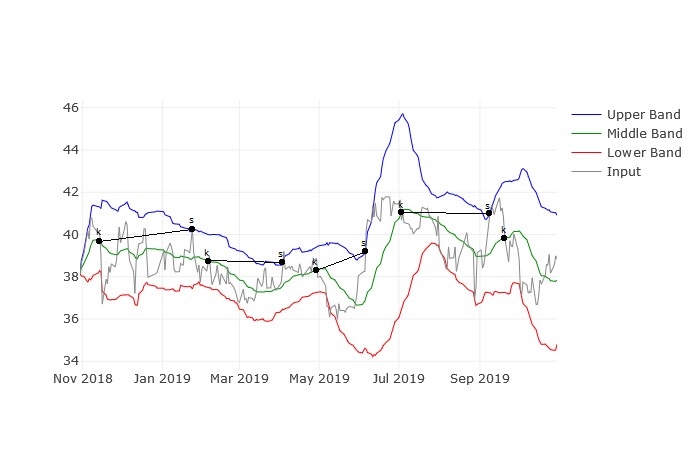
\includegraphics{rysunki/Bollinger Bands_m-u}
    }
    % opis obrazka
    \caption[Wst�gi Bollingera - Przyk�ad 3]{Wykres przedstawiaj�cy Przyk�ad 3: sprzeda� w szczycie cenowym i kupno po wyj�ciu ze szczytu cenowego. Czarnym kropkami zaznaczone s� momenty kupna/sprzeda�y (literka "k" dla kupna, a  "s" dla sprzedarzy).}

    % etykieta
    \label{Wykres wst�g Bollingera}
  \end{center}
\end{figure*}
\subsection{podsumowanie}
Wst�gi Bollingera pozwalaj� na wykrywanie potencjalnych do�k�w cenowych oraz szczyt�w cenowych. Najlepiej sprawdzaj� si� w kr�tkich inwestycjach.

\autsection{Oscylator Stochastyczny}{Agnieszka Wojciechowska}
\subsection{wprowadzenie}
Oscylator stochastyczny jest wska�nikiem, kt�ry pozwala �ledzi� ruchy cen i si�� trendu momentum. 

Omawiany wska�nik zosta� wprowadzony w 1950 r. przez George'a Lana w celu por�wnywania cen zamkni�cia do wszystkich w danym okresie [19]. Oscylator wyst�puje w trzech wersjach: szybkiej, wolnej i pe�nej. Wersja szybka jest najlepsza w zastosowaniu przy analizach kr�tkoterminowych, a wolna do analiz d�ugoterminowych. Pe�na wersja - Stochastic Full czyli STS jest najbardziej uniwersalna ze wszystkich wersji. W�a�nie ta wersja zosta�a zaimplementowana.

\subsection{zasady dzia�ania}
\subsubsection{wz�r}
Wska�nik sk�ada si� z dw�ch linii: linii wolno oscyluj�cej zwanej \%K oraz linii \%D, kt�ra jest 3 okresow� �redni� krocz�c� z \%K. Linia \%K wyznaczana jest na podstawie znajomo�ci ceny zamkni�cia z danego dnia oraz cen najni�szej i najwy�szej z domy�lnie przyj�tych 14 poprzednich sesji zamkni�cia. Z kolei otrzymane warto�ci s� u�redniane i zobrazowane za pomoc� linii \%D. Wyznaczana jest na podstawie �redniej krocz�cej 3 poprzednich sesji z wyznaczonego \%K na dany moment. Okres 3 dniowy jest r�wnie� standardowo przyj�t� warto�ci� u�ywan� dla tego wska�nika. [20]
\begin{equation}
\begin{array}{lll}
\%K & = & 100 \times \frac{C - L_{14}}{H_{14} - L_{14}} \\
\%D & = & EMA_{3}(\%K)
\end{array}
\end{equation}
We wzorze:
\begin{itemize}
\item C - aktualny kurs zamkni�cia 
\item $L_{14}$ - najni�sza cena w przedziale 14 okresowym 
\item $H_{14}$ - najwy�sza cena w przedziale 14 okresowym
\item $EMA_{3}$ - �rednia krocz�ca w przedziale 3 okresowym
\end{itemize}
\begin{figure*}[!h]
  % wy�rodkowanie zawarto�ci pola obrazka
  \begin{center}
    % okienko skaluj�ce:
    %  pierwszy argument szeroko��, drugi wysoko��,
    %  jeden z nich mo�e by� zast�piony ! - zachowanie proporcji obrazka
    %  w taki spos�b mo�emy skalowa� tak�e inne obiekty np. tekst
    \resizebox{1\textwidth}{!}{
      % wstawienie obrazka
      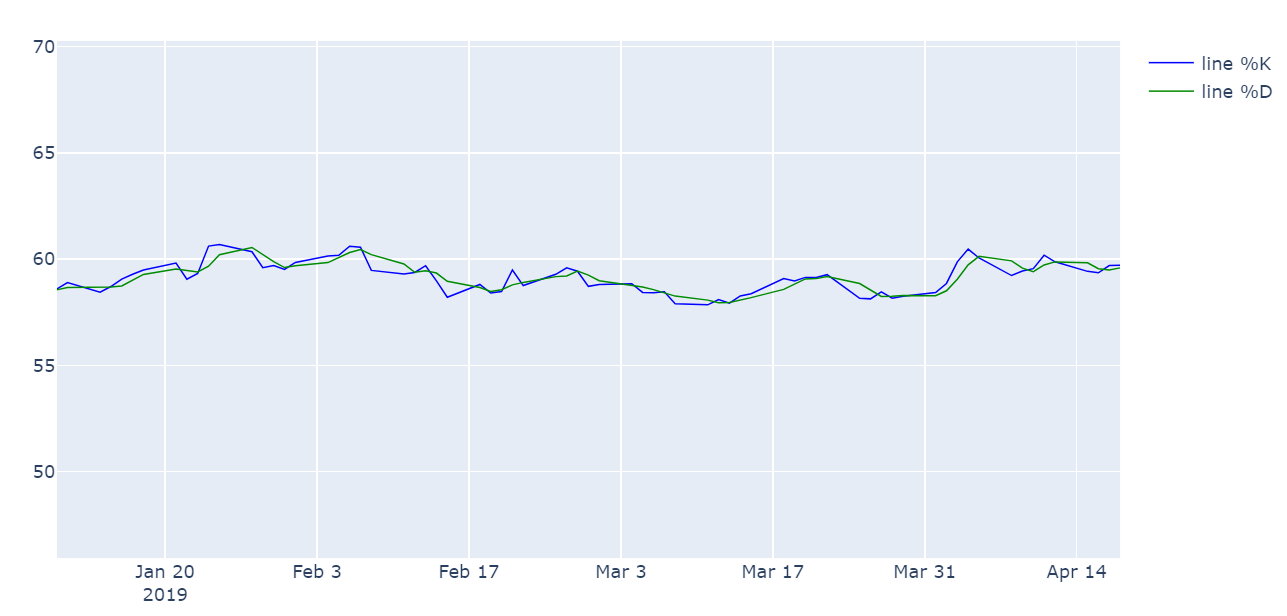
\includegraphics{rysunki/stochastic_oscillator}
    }
    % opis obrazka
    \caption[Oscylator stochastyczny - wykres]{Wykres przedstawia oscylator stochastyczny.}
    % etykieta
    \label{Wykres stochastic oscillator}
  \end{center}
\end{figure*}

\subsubsection{strategia decyzyjna}
Aby analizowa� wskazania oscylatora najpierw nale�y zaznaczy�, �e jego wskazania znajduj� si� w zakresie od 0\% - 100\%. Zakres 0 jest w okolicach najmniejszej warto�ci sygna��w oscylatora stochastycznego, a 100 jest dla najwy�szej warto�ci. Do interpretacji wskaza� jako istotne momenty na wykresie przyjmuje si� standardowo poziom na wysoko�ci 20\% i 80\% wykresu - nazywane poziom 20 i poziom 80. 
\begin{itemize}
    \item Sygna� na kupno akcji - linia \%K przecina w d� poziom 20 
    \item Sygna� na sprzeda� akcji - linia \%K przecina w g�r� poziom 80
\end{itemize}
Poziom 20 nazywany jest te� poziomem wyprzedania, a z kolei poziom 80 to poziom wykupienia. [18]

\subsection{przyk�ady numeryczne}
Zastosowanie i interpretacja oscylatora stochastycznego w praktyce zostanie przedstawiona na dw�ch poni�szych przyk�adach. Do przyk�adu, dla wi�kszej czytelno�ci wykresu zosta�o wybrane przybli�enie warto�ci do zakresu 4 miesi�cy, od stycznia do kwietnia 2019. Ponadto u�yte dane pochodz� z serwisu Stooq. Dane wej�ciowe zosta�y przedstawione na rys. 4.13.
\begin{figure*}[!h]
  % wy�rodkowanie zawarto�ci pola obrazka
  \begin{center}
    % okienko skaluj�ce:
    %  pierwszy argument szeroko��, drugi wysoko��,
    %  jeden z nich mo�e by� zast�piony ! - zachowanie proporcji obrazka
    %  w taki spos�b mo�emy skalowa� tak�e inne obiekty np. tekst
    \resizebox{1\textwidth}{!}{
      % wstawienie obrazka
      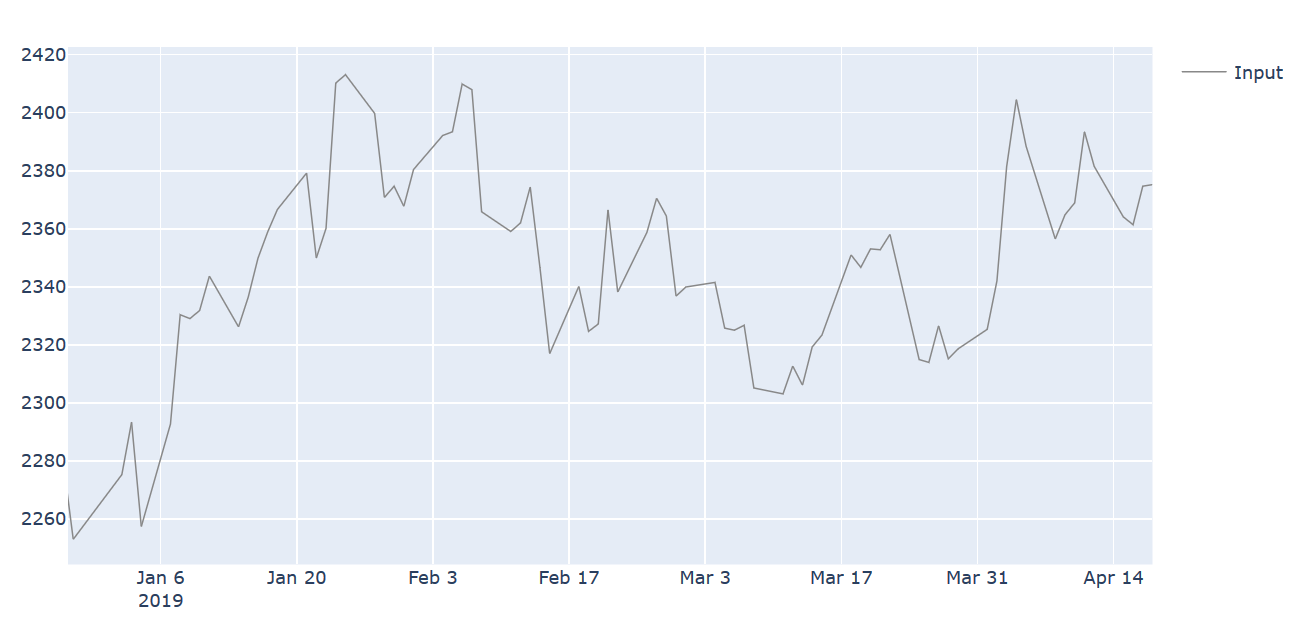
\includegraphics{rysunki/input_MACD_stochastic}
    }
    % opis obrazka
    \caption[oscylator stochastyczny - sygnal wejsciowy]{Wykres przedstawia sygna� wej�ciowy do przedstawionych poni�ej przyk�ad�w.}
    % etykieta
    \label{oscylator stochastyczny - sygnal wejsciowy}
  \end{center}
\end{figure*}

\subsubsection{Przyk�ad 1: sygna� kupna}
Dla sygna�u kupna linia \%K przecina w d� poziom 20\% swojego zakresu. Dla zastosowanego przedzia�u czasu, w tym przyk�adzie mo�na zaobserwowa� wygenerowane trzy przyk�ady sygna��w kupna: 15 lutego, 5 marca oraz 26 marca. 
\begin{figure*}[!h]
  % wy�rodkowanie zawarto�ci pola obrazka
  \begin{center}
    % okienko skaluj�ce:
    %  pierwszy argument szeroko��, drugi wysoko��,
    %  jeden z nich mo�e by� zast�piony ! - zachowanie proporcji obrazka
    %  w taki spos�b mo�emy skalowa� tak�e inne obiekty np. tekst
    \resizebox{1\textwidth}{!}{
      % wstawienie obrazka
      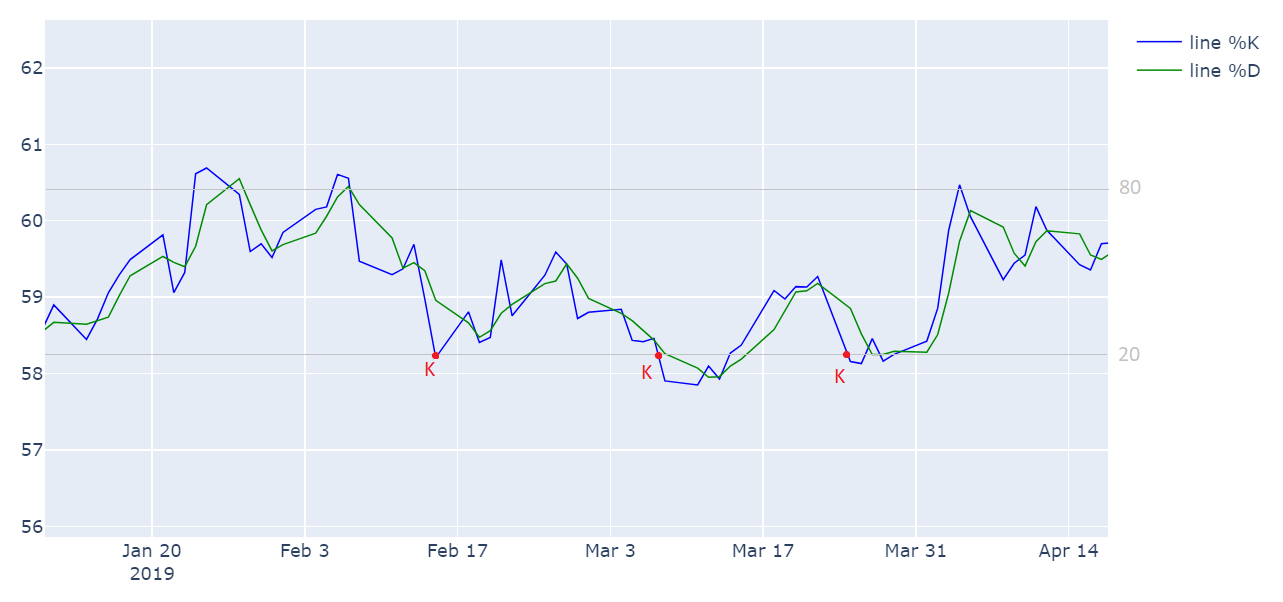
\includegraphics{rysunki/stochastic_oscillator_kup}
    }
    % opis obrazka
    \caption[Oscylator stochastyczny - strefa wykupienia]{Wykres przedstawia momenty wej�cia w stref� wykupienia (K) wygenerowane przez oscylator stochastyczny.}
    % etykieta
    \label{Wykres stochastic oscillator}
  \end{center}
\end{figure*}

Efektem jaki mo�na zaobserwowa� jest to, �e po przekroczeniu poni�ej poziomu 20\% wska�nik wszed� w stref� "wykupienia". Nie zawsze jest to jednak pewny sygna�, poniewa� wska�nik mo�e znajdowa� si� w tej strefie przez pewnien czas - wtedy warto rozwa�y� zmiejszenie poziomu do np. 90\%. W tym przyk�adzie wska�nik w dw�ch przypadkach znajdowa� si� przez d�u�szy czas w strefie wykupienia. By�o to od 5 marca do 14 marca oraz kr�tszy okres od 26 marca do 27 marca.

\subsubsection{Przyk�ad 2: sygna� sprzeda�y}
Dla sygna�u sprzeda�y linia \%K przecina w g�r� poziom 80\% swojego zakresu. Dla zastosowanego przedzia�u czasu, w tym przyk�adzie mo�na zaobserwowa� wygenerowane trzy przyk�ady sygna��w sprzeda�y: 25 stycznia, 6 lutego oraz 4 kwietnia.
\begin{figure*}[!h]
  % wy�rodkowanie zawarto�ci pola obrazka
  \begin{center}
    % okienko skaluj�ce:
    %  pierwszy argument szeroko��, drugi wysoko��,
    %  jeden z nich mo�e by� zast�piony ! - zachowanie proporcji obrazka
    %  w taki spos�b mo�emy skalowa� tak�e inne obiekty np. tekst
    \resizebox{1\textwidth}{!}{
      % wstawienie obrazka
      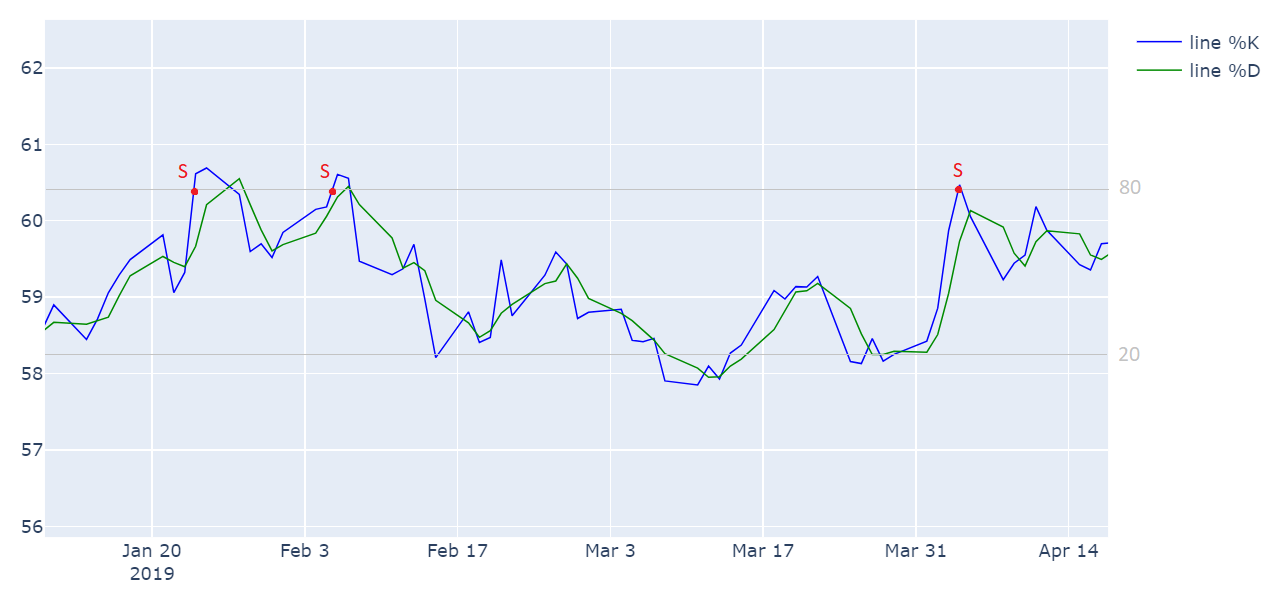
\includegraphics{rysunki/stochastic_oscillator_sprzedaj}
    }
    % opis obrazka
    \caption[Oscylator stochastyczny - strefa wyprzedania]{Wykres przedstawia momenty wej�cia w stref� wyprzedania (S) wygenerowane przez oscylator stochastyczny.}
    % etykieta
    \label{Wykres stochastic oscillator}
  \end{center}
\end{figure*}

Po przekroczeniu powy�ej poziomu 80\% wska�nik wszed� w stref� "wyprzedania". Tak jak dla sygna�u kupna warto pami�ta� i przetestowa� jak wska�nik zachowuje si� powy�ej tego poziomu i dostosowa� indywidualnie parametry. Dla tego przyk�adu wska�nik znajdowa� si� w strefie "wyprzedania" d�u�ej ni� jeden dzie� w dw�ch przypadkach: od 25 stycznia do 28 stycznia oraz od 6 lutego do 7 lutego.

\subsection{podsumowanie}
Oscylator stochastyczny jest �atwy w u�yciu i skuteczny po dostosowaniu odpowiednich parametr�w do danego typu rynku, ze wzgl�du na mo�liwo�� dopasowania odpowiedniej wersji oscylatora. Najcz�ciej u�ywany jest przez inwestor�w do analizy interwa�u dziennego przy du�ej ilo�ci wyra�nych sygna��w. 

\autsection{Wska�nik zagregowany}{Mateusz Rutkiewicz}
Wska�nik zagregowany sk�ada si� z $N$ poprzednich wska�nik�w. Jest on sum� odpowiednich wag przemno�onych przez znormalizowan� warto�� wynikaj�c� z warto�ci wyznaczonych przez poprzedni wska�nik (np. MACD). Dodatkow� warto�ci� pojawiaj�c� si� we wzorze jest warto�� progowa $\omega_0$, kt�r� mo�na interpretowa� jako tendencj� do kupna lub sprzeda�y. Je�eli jest ona ujemna, nasz wska�nik b�dzie wykazywa� mniejsz� tendencj� do kupna i pozosta�e warto�ci b�d� musia�y by� wi�ksze, �eby pokaza� sygna� do kupna. 
\begin{equation}
y = \omega_0 + \sum^N_{i = 1}(\alpha_i\cdot\omega_i)
\end{equation}
\subsection{Normalizacja wska�nik�w}
Do normalizacji wska�nik�w wykorzystujemy funckje aktywacyjne popularne w sieciach neurnowych. Funkcje aktywacyjne, kt�re planujemy wykorzysta� maj� nast�puj�ce cechy:
\begin{itemize}
    \item Przyjmuj� warto�ci w ca�ej dziedzinie liczb rzeczywistych ${\rm I\!R}$
    \item Warto�ci zwracane s� w przedzia�ach $(-1, 1)$ albo $(0, 1)$
    \item S� ci�g�e i rosn�ce
\end{itemize}
W naszym przypadku wykorzystujemy funkcj� nazywaj�c� si� sigmoid. Wagi pozwalaj� stwierdzi� jak wa�na ma by� decyzja danego wska�nika i w przypadku tego wska�nika, je�eli warto�� naszego zagregowanego wska�nika jest wi�ksza ni� 0.5, jest to sygna� do kupna, a je�eli jest mniejsza ni� 0, sygna� do sprzeda�y. W przeciwnym razie algorytm odczekuje.
\subsubsection{Normalizacja MACD}
Do znormalizowania warto�ci zwracanych wska�nik MACD wykorzystamy po prostu ro�nic� pomi�dzy warto�ci� $MACD$ i $signal$.
\begin{equation}
\alpha_{MACD}(X) = MACD_{(12, 26)}(X) - signal_9(X)
\end{equation}
\subsubsection{Normalizacja Wst�g Bollingera}
Do znormalizowania Wst�g Bollingera wykorzystamy opracowany przez samego Bollingera w wiosn� 2010 r. wska�nik bezpo�rednio bazuj�cy na Wst�gach Bollingera - \%b.
\begin{equation}
\alpha_{\%b}(X) = (X - lower \: band) / (upper \: band - lower \: band)
\end{equation}
\subsection{Algorytm Genetyczny}
\subsubsection{Opis}
Algorytm genetyczny jest algorytmem heurystycznym do znajdowania prawie optymalych rozwi�za� w sytuacjach, gdy szukanie rozwi�zania optymalnego jest trudne i samo rozwi�zanie prawie optymalne nas satysfakcjonuje. Algorytm jest wzorowany na dzia�aniu ewolucji genetycznej u zwierz�t w naturze. 

\subsubsection{S�owniczek poj��}
W algorytmie genetycznym wykorzystuje si� nast�puj�ce poj�cia:
\begin{itemize}
	\item Chromosom - reprezentacja rozwi�zania problemu
	\item Osobnik - inne okre�lenie na chromosom
	\item Gen - pojedy�cza waga w chromosomie
	\item Fitness - warto�� oznaczaj�ca dopasowanie chromosomu do rozwi�zania naszego problemu (przyk�adowo im wy�sza jest warto�� fitness, tym chromosom lepiej rozwi�zuje nasz problem)
	\item Selekcja - wyb�r najlepiej dopasowanych osobnik�w
	\item Krzy�owanie - tworzenie nowego osobnika poprzez mieszanie gen�w dw�ch innych osobnik�w
	\item Mutacja - zmiana genu na inny gen u kt�rego� z osobnik�w
	\item Pokolenie - pula osobnik�w w danej iteracji algorytmu
\end{itemize}

\subsubsection{Dzia�anie}
Pierwszym krokiem algorytmu genetycznego jest wygenerowanie pierwszego pokolenia. Wykonuje si� to poprzez losow� generacj� gen�w dla ka�dego nowego osobnika. Nast�pnymi krokami s�: obliczenie warto�ci fitness dla ka�dego z osobnik�w oraz selekcja osobnik�w na podstawie tej warto�ci. W tym momencie mo�emy zapami�ta� najlepszego do tej pory osobnika. Wa�ne, by zrobi� to przed mutacj�, gdy� w wyniku mutacji geny mog� si� zmieni�. Gdy osobniki zostan� wybrane, ca�a reszta jest usuwana, a na ich miejsce tworzone s� nowe osobniki poprzez krzy�owanie dw�ch losowo wybieranych osobnik�w. Powsta�e w ten spos�b pokolenie mo�e znacz�co r�ni� pomi�dzy r�nymi uruchomieniami algorytmu, nawet je�li pokolenie, z kt�rego te osobniki s� generowane jest takie same, jednak krzy�uj�c tak osobniki ze sob� mamy du�� szans�, �e kt�ry� z nowo powsta�ych osobnik�w b�dzie jeszcze lepiej dopasowany do problemu (szukamy w ten spos�b lokalnego najlepszego rozwi�zania). Przedostatnim krokiem jest mutacja gen�w, kt�ra dla ka�dego osobnika odbywa si� z losowym prawdopodobie�stwem (cz�� osobnik�w mo�e nie zmutowa�). Naszym celem jest znalezienie najlepszego rozwi�zania globalnego, jednak krzy�owanie zbli�a nas jedynie do najlepszego lokalnego rozwi�zania dla obecnego pokolenia. Mutacje s� rozwi�zaniem tego problemu sprawiaj�c, �e rozszerzamy spektrum poszukiwa�. Wa�nym parametrem tutaj jest prawdopodobie�stwo wyst�powania mutacji. Przy zbyt du�ym algorytm b�dzie dzia�a� w spos�b zbyt przypadkowy, a przy zbyt ma�ym - przez bardzo d�ugie czasy b�dziemy pozostawa� w lokalnym najlepszym rozwi�zaniu. Najcz�ciej stosowane prawdopodobie�stwo na mutacj� genu w algorytmach genetycznych to pomi�dzy 0.2\% a 0.5\%. Czasami sama mutacja to zama�o, poniewa� szansa na to, �e dany osobnik przetrwa w selekcji po mutacji jest ma�a, wi�c w bardziej z�o�onych algorytmach genetycznym symuluje si� podzia� na gatunki sprawiaj�c, �e nawet najmniej dopasowany osobnik, je�eli wyj�tkowo r�ni si� od pozosta�ych, mo�e przetrwa�, daj�c mu w ten spos�b szans� do znalezienia lokalnego najlepszego rozwi�zania dla tego osobnika. Po mutacji sprawdzamy warunek zako�czenia algorytmu (np. liczb� iteracji, kt�r� mieli�my wykona�) i wracamy do kroku drugiego kroku algorytmu (obliczania warto�ci fitness) , je�eli warunek nie jest spe�niony.

\subsection{Podsumowanie}
Uzyskany w ten spos�b wska�nik w wi�kszo�ci przypadk�w podejmowa� tylko 2 decyzje, albo kupowa� na samym pocz�tku akcje i ich nie sprzedawa� do ko�ca, albo w og�le nie kupowa� akcji, przez co nic nie traci�.

\begin{figure*}[!h]
\centering
\subfloat
{
    \resizebox{0.5\textwidth}{!}{
      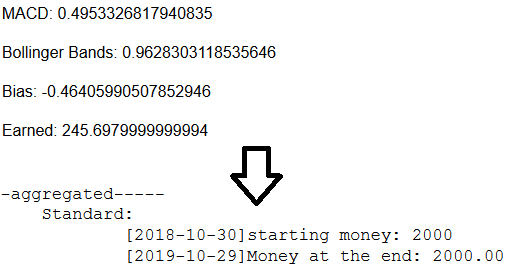
\includegraphics{rysunki/wskaznik_zagregowany1}
    }
}
\subfloat
{
    \resizebox{0.5\textwidth}{!}{
      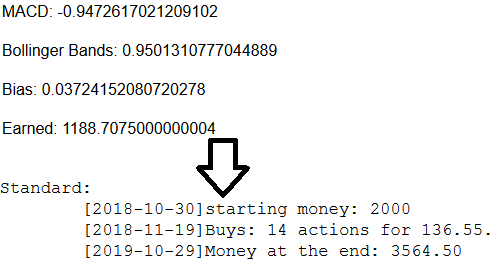
\includegraphics{rysunki/wskaznik_zagregowany2}
    }
}
\caption{Wynik wska�nika zagregowanego}
\end{figure*}

\autsection{Por�wnanie wska�nik�w}{Mateusz Rutkiewicz}
Ka�dy z poni�szych przypadk�w jest testowany na tym samym zbiorze danych z okresu ok. roku. Pocz�tkowa kwota to 2000 z�. Na podstawie wynik�w wska�nika podejmowane s� decyzje o kupnie lub sprzedarzy, po czym na samym ko�cu wszystkie akcje s� sprzedawane za ostatni� cen� i liczona jest uzyskana kwota. Przeprowadzono testy zaimplementowanych symulacji inwestycji wska�nik�w, to jest symulacji MACD i wst�g Boillingera.
\begin{figure*}[!h]
\centering
\subfloat[CD Project SA]
{
    \resizebox{0.33\textwidth}{!}{
      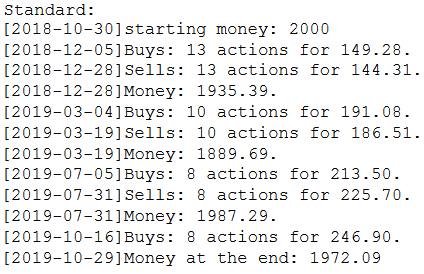
\includegraphics{rysunki/MACD_result1}
    }
}
\subfloat[AmRest Holdings SE]
{
    \resizebox{0.33\textwidth}{!}{
      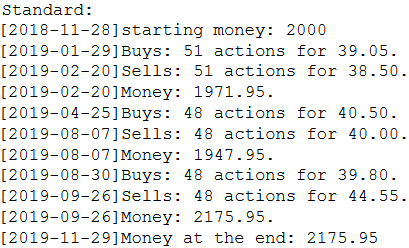
\includegraphics{rysunki/MACD_result2}
    }
}
\subfloat[Grupo Santander]
{
    \resizebox{0.33\textwidth}{!}{
      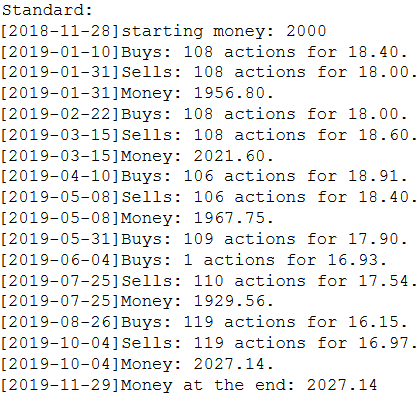
\includegraphics{rysunki/MACD_result3}
    }
}
\caption{Wynik wska�nika MACD - powy�sze rysunki przedstawiaj� wyniki testu wska�nika MACD na akcjach 3 sp�ek z okresu jednego roku. Dla CD Project SA wska�nik wykaza� si� ma�� strat�, dla Amrest Holdings SE pod koniec uda�o mu si� odbi� i zarobi� 175.95 z�, natomiast dla Grupo Santander znowu na koniec zysk by� na niskim poziomie.}
\end{figure*}

\begin{figure*}[!h]
\centering
\subfloat
{
    \resizebox{0.33\textwidth}{!}{
      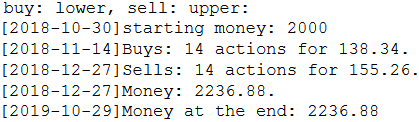
\includegraphics{rysunki/BB_lu_result1}
    }
}
\subfloat
{
    \resizebox{0.33\textwidth}{!}{
      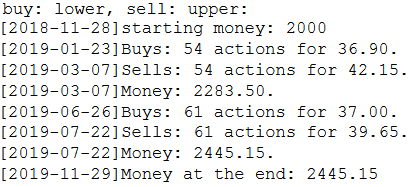
\includegraphics{rysunki/BB_lu_result2}
    }
}
\subfloat
{
    \resizebox{0.33\textwidth}{!}{
      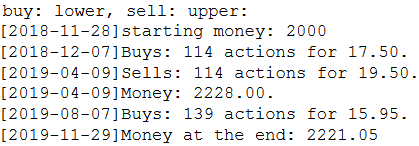
\includegraphics{rysunki/BB_lu_result3}
    }
}
\caption{Wynik Wst�g Bollingera dla strategii kup w do�ku cenowym, sprzedaj w szczycie cenowym - powy�sze rysunki przedstawiaj� wyniki testu Wst�g Bollingera na akcjach 3 sp�ek z okresu 2018 - 2019. Tutaj wida�, �e dla podanych przyk�ad�w wska�nik daje pozytywne efekty.}
\end{figure*}

\begin{figure*}[!h]
\centering
\subfloat
{
    \resizebox{0.33\textwidth}{!}{
      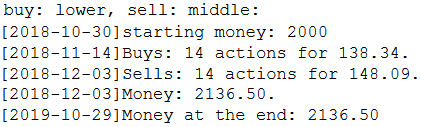
\includegraphics{rysunki/BB_lm_result1}
    }
}
\subfloat
{
    \resizebox{0.33\textwidth}{!}{
      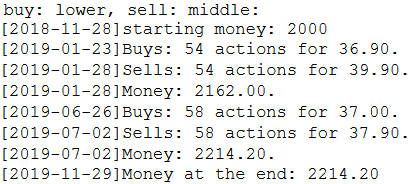
\includegraphics{rysunki/BB_lm_result2}
    }
}
\subfloat
{
    \resizebox{0.33\textwidth}{!}{
      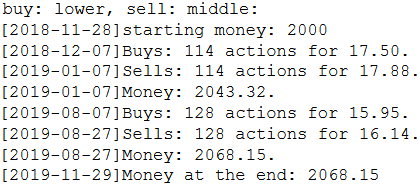
\includegraphics{rysunki/BB_lm_result3}
    }
}
\caption{Wynik Wst�g Bollingera dla strategii kup w do�ku cenowym, sprzedaj po wyj�ciu z do�ku cenowego  - powy�sze rysunki przedstawiaj� wyniki testu Wst�g Bollingera na akcjach 3 sp�ek z okresu 2018 - 2019. Wska�nik wypad� podobnie jak poprzednio, tylko zarobki by�y o ok. 50\% mniejsze.}
\end{figure*}

\begin{figure*}[!h]
\centering
\subfloat
{
    \resizebox{0.33\textwidth}{!}{
      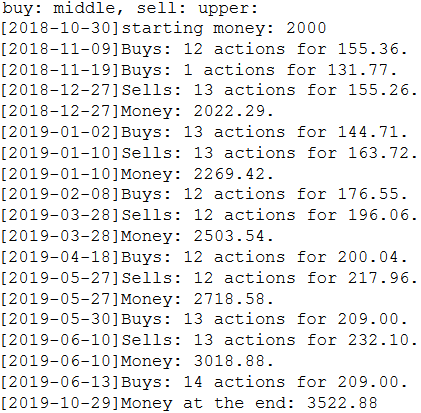
\includegraphics{rysunki/BB_mu_result1}
    }
}
\subfloat
{
    \resizebox{0.33\textwidth}{!}{
      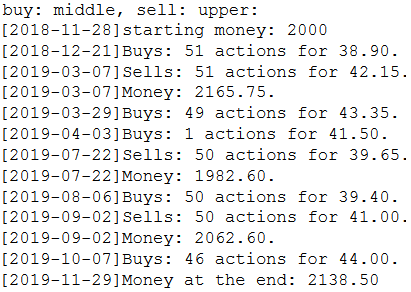
\includegraphics{rysunki/BB_mu_result2}
    }
}
\subfloat
{
    \resizebox{0.33\textwidth}{!}{
      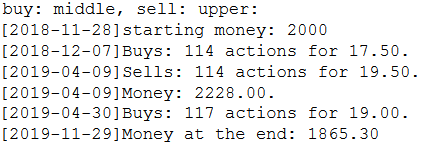
\includegraphics{rysunki/BB_mu_result3}
    }
}
\caption{Wynik Wst�g Bollingera dla strategii kup po wyj�ciu ze szczytu cenowego, sprzedaj po wej�ciu na szczyt cenowy- powy�sze rysunki przedstawiaj� wyniki testu Wst�g Bollingera na akcjach 3 sp�ek z okresu 2018 - 2019. Dla akcji CD Project SA strategia ta da�a zaskakuj�co dobry wynik. Uda�o si� powi�kszy� kapita� o 75\%. Dla AmRest Holdings SE natomiast zyskano niewiele, a dla Grupo Santander strategia przynios�a straty.}
\end{figure*}

Dla podanych przyk�ad�w Wst�gi Bollingera da�y o wiele lepszy efekt ni� MACD. W szczeg�lno�ci strategia kup w do�ku cenowym i sprzedaj w szczycie cenowym. Du�ym zaskoczeniem jest tutaj strategia kup po wyj�ciu ze szczytu cenowego i sprzedaj w szczycie cenowym dla CD Project SA. By� mo�e akcje tej sp�ki kr��� g��wnie pomi�dzy w�a�nie tymi dwoma strategicznymi punktami, a Wst�gi Bollingera akurat dobrze to wykrywaj�.
%\input{rozdzialy/przyklad_rozdzialu_3.tex}

% itd...

% ---------------------- Bibliografia -----------------------
\bibliographystyle{plain}                       % styl bibliografii
\begin{thebibliography}{3}                      % pocz�tek �rodowiska
\addcontentsline{toc}{chapter}{Wykaz literatury}    % dodaje bibliografi� do spisu tre�ci

\small              % spisy i bibliografie sk�adamy mniejszym stopniem pisma
% przyk�adowy wpis
    \bibitem{BiznesRadar.pl}      % \bibitem{etykieta}
BiznesRadar.pl 
% nast�pna pozycja
    \bibitem{Kahn}
Michael N. Kahn: \emph{Analiza techniczna}, wyd. GAB, 2018
% nast�pna pozycja
    \bibitem{Majchrowski}
Dr Klaudiusz Majchrowski: \emph{Wyk�ad dla Elekroradiologii, Podstawy elektroniki i akustyki}, www.ur.edu.pl/file/71671/Podstawy
% nast�pna pozycja
    \bibitem{Wiki_sygnal}
Wikipedia: \emph{Sygna�}, pl.wikipedia.org/wiki/Sygna\%C5\%82\#Zastosowania
% nast�pna pozycja
    \bibitem{Erhard}
Jan Erhard: \emph{Technika cyfrowa - podstawy}, www.livesound.pl/tutoriale/3938-technika-cyfrowa-podstawy.-zacznijmy-od-poczatku.
% nast�pna pozycja
    \bibitem{lomiowka}
Szko�a w Mil�wce: \emph{Zapis analogowy i cyfrowy d�wi�ku}, www.lomilowka.pl/pliki/1\_zapis\_dzwieku\_pdf-9092.pdf
% nast�pna pozycja
    \bibitem{wiki_dyskretyzacja}
Wikipedia: \emph{Dyskretyzacja}, pl.wikipedia.org/wiki/Dyskretyzacja\_(statystyka)
% nast�pna pozycja
    \bibitem{wiki_kwantyzacja}
Wikipedia: \emph{Kwantyzacja}, pl.wikipedia.org/wiki/Kwantyzacja\_(technika)\#Kwantyzacja\_sygna\%C5\%82u\_analogowego
% nast�pna pozycja
    \bibitem{Labaj}
Weronika �abaj: \emph{Sygna�}, zasoby.open.agh.edu.pl/~10swlabaj/sygnal/sygnal2.html
% nast�pna pozycja
    \bibitem{Jozwiak}
Arkadiusz J�wiak: \emph{3 sposoby jak wykorzysta� �rednie krocz�ce}, comparic.pl/3-sposoby-wykorzystac-srednie-kroczace-tradingu/
% nast�pna pozycja
    \bibitem{edukacja_gieldowa}
Strona edukacja gie�dowa: \emph{Analiza techniczna}, www.edukacjagieldowa.pl/gieldowe-abc/analiza-techniczna/
% nast�pna pozycja
    \bibitem{Google_Play}
Google Play: \emph{Aplikacja BiznesRadar}, play.google.com/store/apps/details?id=com.Android.BiznesRadar\&hl=pl
% nast�pna pozycja
    \bibitem{tradersarea}
Strona tradersarea: \emph{MACD jako jeden z najpopularniejszych wska�nik�w}, tradersarea.pl/macd-jako-jeden-z-najpopularniejszych-wskaznikow/
% nast�pna pozycja
    \bibitem{edu_gield_macd}
Strona edukacja gie�dowa: \emph{Krzywa MACD}, https://www.edukacjagieldowa.pl/gieldowe-abc/analiza-techniczna/narzedzia-analizy-technicznej/krzywa-macd/
% nast�pna pozycja
    \bibitem{TradingView}
Strona TradingView: \emph{MACD, zbie�no��/ rozbie�no�� �rednich ruchomych}, www.tradingview.com/wiki/MACD\_(Moving\_Average\_Convergence/Divergence)/pl
% nast�pna pozycja
    \bibitem{admiralmarkets}
Strona admiralmarkets: \emph{Wska�nik MACD - najpopularniejszy ze wska�nik�w}, https://admiralmarkets.pl/education/articles/forex-indicators/wskaznik-macd
% nast�pna pozycja
    \bibitem{stooq}
Serwis stooq: www.stooq.pl
% nast�pna pozycja
    \bibitem{edu_gield_stoch}
Strona edukacja gie�dowa: \emph{Oscylator stochastyczny}, www.edukacjagieldowa.pl/gieldowe-abc/analiza-techniczna/narzedzia-analizy-technicznej/oscylator-stochastyczny/
% nast�pna pozycja
    \bibitem{admiralmarkets_stoch}
Strona admiralmarkets: \emph{Oscylator Stochastyczny - Handel w Oparciu o Stochastic}, admiralmarkets.pl/education/articles/forex-indicators/oscylator-stochastyczny
% nast�pna pozycja
    \bibitem{tradersarea_stoch}
Strona tradersarea: \emph{Oscylator Stochastyczny Stochastic}, tradersarea.pl/oscylator-stochastyczny-stochastic/
% nast�pna pozycja
    \bibitem{zielinski}
Tomasz P. Zieli�ski: \emph{Cyfrowe przetwarzanie sygna��w}, wyd. Komunikacji i ��czno�ci sp. z.o.o Warszawa 2005, 2009
% nast�pna pozycja
    \bibitem{numba}
Numba: \emph{installation}, numba.pydata.org/numba-doc/dev/user/installing.html
% nast�pna pozycja
    \bibitem{rpubs_installation}
Mohammad Shadan: \emph{Python - Install Anaconda, Jupyter Notebook}, rpubs.com/mohammadshadan/installanaconda
\vspace{0.8cm} \\
Wszystkie adresy stron www s� aktualne na dzie� 01.12.2019r.
\end{thebibliography}                           % koniec �rodowiska % dodanie pliku bibliografii
% -----------------------------------------------------------

%------------------------------------------------------------
%	Dodanie wykazu rysunk�w oraz tabeli

\renewcommand{\baselinestretch}{1.0}\normalsize	% interlinia w sekcji wykaz�w
\addcontentsline{toc}{chapter}{\listfigurename}	% dodanie wykazu rysunk�w do spisu tre�ci
\listoffigures									% generacja wykazu rysunk�w

\addcontentsline{toc}{chapter}{\listtablename}	% dodanie wykazu tabel do spisu tre�ci
\listoftables									% generacja wykazu tabel
\renewcommand{\baselinestretch}{1.3}\normalsize	% powr�t do interlinii 1.5


% ---------------------- DODATKI -----------------------
\chapter*{Dodatek A}
\addcontentsline{toc}{chapter}{Dodatek A}
% Zale�nie od dodatku, zaleca si� dodawa� dodatki jako
% dokumenty PDF
% \includepdf{dodatki/dodatek1.pdf}

% -----------------------------------------------------------
\end{document}
%------------------------------------------------------------
			 	%	Koniec pracy dyplomowej  %
%------------------------------------------------------------
